\documentclass[Bachelor, UKenglish, ngerman]{scrbook}
%------------------------------------------------------------------------------
% This file contains a skeleton thesis for
% a Physics or Astronomy Institute in the University of Bonn

% Specify the thesis type as an option: PhD, Master, Diplom, Bachelor
% Specify the thesis stage as an option: Draft (default), Submit, Final, PILibrary

% Specify the language(s) in the class and then use babel.
% If you need more than one language, give the default language last,
% e.g. ngerman, UKenglish for a thesis in British (UK) English where you want
% to be able to set the language to German for some part of it.

%------------------------------------------------------------------------------
% Pass TeX Live version to the package
% Use command pdflatex --version to find out which version you are running
% Add option backref=false when your thesis is ready to turn off back-referencing
% in your bibliography
\usepackage[texlive=2019]{ubonn-thesis}
% Adjustments to standard biblatex style
\usepackage{ubonn-biblatex}

% Glossary package
% \usepackage[acronym,toc,nosuper]{glossaries}
% TikZ packages and libraries
% \usepackage{tikz}
% \usepackage{tikz-3dplot}
% \usepackage{pgfplots}
% \usetikzlibrary{positioning,shapes,arrows}
% \usetikzlibrary{decorations.pathmorphing}
% \usetikzlibrary{decorations.markings}
\usepackage{thesis_defs}

%Eigene Pakete, z.B. fuer Gnuplot, wrapfigure:
\usepackage{wrapfig}
\usepackage{graphicx}
\usepackage{color}
\usepackage{epstopdf}
\pdfminorversion=7
%------------------------------------------------------------------------------
% Instead of colouring  links, cites, table of contents etc.
% put them in a coloured box for the screen version.
% This is probably a good idea when you print your thesis.
% \hypersetup{colorlinks=false,
%   linkbordercolor=blue,citebordercolor=magenta,urlbordercolor=darkgreen
% }

%------------------------------------------------------------------------------
% When writing your thesis it is often helpful to have the date and
% time in the output file. Comment this out for the final version.
\ifoot[\today{} \thistime]{\today{} \thistime}

% In order to check if your labels are referenced try the refcheck package
% \usepackage{refcheck}

%------------------------------------------------------------------------------
% biblatex is included by ubonn-thesis. Look there for the settings used.
% See the options for settings that can be changed easily.
% For further changes copy the \RequirePackage[...]{biblatex} here
% and include ubonn-thesis with the option biblatex=false.

% Specify the bibliography files here and not at the end!
% Use standard_refs-bibtex if you use bibtex or bibtex8
% and standard_refs-biber  if you use biber
%\addbibresource{bib/thesis_refs.bib}
%\addbibresource{bib/standard_refs-biber.bib}
\addbibresource{refsgrosschristiane.bib}

%------------------------------------------------------------------------------
% The following definitions are used to produce the title pages
% needed at various stages
\newcommand{\thesistitle}{Monte-Carlo Simulation eines statistischen Modells auf einem Parallelrechner}
\newcommand*{\thesisauthor}{Christiane Franziska Groß}
\newcommand*{\thesistown}{Dortmund}
\renewcommand*{\InstituteName}{\HISKP}
\renewcommand*{\inInstitute}{\inHISKP}
\renewcommand*{\InstituteAddress}{\HISKPaddress}
% Adjust \thesisreferee...text depending on male/female referee
\newcommand*{\thesisrefereeonetext}{1.\ Gutachter}
\newcommand*{\thesisrefereeone}{Prof.\ Dr.\ Carsten Urbach}
\newcommand*{\thesisrefereetwotext}{2.\ Gutachterin}
\newcommand*{\thesisrefereetwo}{}
% Date when thesis was submitted (Master/Diplom)
% Year or Month, Year when thesis was submitted (PhD)
\newcommand*{\thesissubmit}{XX.YY.2020}
% \newcommand*{\thesissubmit}{Month 2020}
% Date of thesis examination (PhD)
\newcommand*{\thesispromotion}{XX.YY.2020}
% Month and year of the final printed version of the thesis
\newcommand*{\thesismonth}{Juli}
\newcommand*{\thesisyear}{2020}
\newcommand*{\thesisnumber}{BONN-IR-2020-XXX}

%------------------------------------------------------------------------------
% The abstract is only needed for the printed version and should be in
% English regardless of the language of the thesis
\newcommand{\thesisabstract}{%
  \begin{otherlanguage}{UKenglish}
    This is your thesis abstract. It may be in a language that is
    different from the rest of your thesis.
  \end{otherlanguage}
}

%------------------------------------------------------------------------------
% \includeonly can be used to select which chapters you want to process
% A simple \include command just inserts a \clearpage before and after the file
% Note that \includeonly can be quite picky! Do not forget to put a
% comma after the filename, otherwise it will simply be ignored!
% \includeonly{%
%   thesis_intro,
%   thesis_appendix,
%   thesis_acknowledge
% }

%------------------------------------------------------------------------------
% Give a list of directories where figures can be found. Do not leave
% any spaces in the list and end the directory name with a /
\graphicspath{%
%  {figs/}%
%  {figs/cover/}%
	{Bilder/}
}

%------------------------------------------------------------------------------
% Make a glossary and a list of acronyms
% \makeglossaries

% Glossary entries
% \input{thesis_glossary}

% Draft version - add the word DRAFT on the cover pages
\ifthenelse{\equal{\ThesisVersion}{Draft}}{%
  \usepackage{background}
  \ifthenelse{\texlive < 2013}{%
    \SetBgContents{DRAFT}
    \SetBgColor{blue!30}
  }{%
    \backgroundsetup{contents=DRAFT, color=blue!30}
  }
}

%------------------------------------------------------------------------------
\begin{document}

% Cover page of thesis - this is only needed for the printed final
% version to be submitted to the department library
% Do not use this page for thesis submission to the Prüfungsamt or Promotionsbüro!
\ifthenelse{\equal{\ThesisVersion}{PILibrary}}{%
  \typeout{Document \jobname, Info: PI library version of thesis}
  \input{../cover/\ThesisType_Cover}
}{}

% Start counting pages from the title page
\frontmatter
% Dedication has to come before \maketitle
% \dedication{Dedicated to no one}

% Select the correct title page(s)
\ifthenelse{\equal{\ThesisType}{Unknown}}{%
  \typeout{Document \jobname, Error: Unknown thesis type - no title page printed}
}{%
  % Bachelor thesis only has one title page
  \ifthenelse{\equal{\ThesisType}{Bachelor}}{%
    \typeout{Document \jobname, Info: Bachelor thesis}
    \input{cover/\ThesisType_Title}
  }{%
    \ifthenelse{\equal{\ThesisVersion}{Final} \OR \equal{\ThesisVersion}{PILibrary}}{%
      % Final and PI library versions
      \typeout{Document \jobname, Info: Final version of a \ThesisType  thesis}
      \input{cover/\ThesisType_Final_Title}
    }{% Submission and draft versions
      \input{cover/\ThesisType_Submit_Title}
      \typeout{Document \jobname, Info: Draft/submission version of a \ThesisType  thesis}
    }
  }
}

\pagestyle{scrplain}

%------------------------------------------------------------------------------
% You can add your acknowledgements here - don't forget to also add
% them to \includeonly above
%%------------------------------------------------------------------------------
\chapter*{Acknowledgements}
\label{sec:ack}
%------------------------------------------------------------------------------

I would like to thank ...

You should probably use \texttt{\textbackslash chapter*} for
acknowledgements at the beginning of a thesis and
\texttt{\textbackslash chapter} for the end.

%%% Local Variables: 
%%% mode: latex
%%% TeX-master: "../mythesis"
%%% End: 


\tableofcontents

\mainmatter
\pagestyle{scrheadings}

% Turn off DRAFT for the following pages
\ifthenelse{\equal{\ThesisVersion}{Draft}}{%
  \ifthenelse{\texlive < 2013}{%
    \SetBgContents{}
  }{%
    \backgroundsetup{contents={}}
  }
}{}

%------------------------------------------------------------------------------
% Add your chapters here - don't forget to also add them to \includeonly above
%% !TEX root = mythesis.tex

%==============================================================================
\chapter{Introduction}
\label{sec:intro}
%==============================================================================

The introduction usually gives a few pages of introduction to the
whole subject, maybe even starting with the Greeks.

For more information on \LaTeX{} and the packages that are available
see for example the books of Kopka~\cite{kopka04} and Goossens et
al~\cite{goossens04}.

A lot of useful information on particle physics can be found in the
\enquote{Particle Data Book}~\cite{pdg2010}.

I have resisted the temptation to put a lot of definitions into the
file \texttt{thesis\_defs.sty}, as everyone has their own taste as
to what scheme they want to use for names.
However, a few examples are included to help you get started:
\begin{itemize}
\setlength{\itemsep}{0pt}\setlength{\parskip}{0pt}
\item cross-sections are measured in \si{\pb} and integrated
  luminosity in \si{\invpb};
\item the \KoS is an interesting particle;
\item the missing transverse momentum, \pTmiss, is often called
  missing transverse energy, even though it is calculated using a vector sum.
\end{itemize}
Note that the examples of units assume that you are using the
\textsf{siunitx} package.

It also is probably a good idea to include a few well formatted
references in the thesis skeleton. More detailed suggestions on what
citation types to use can be found in the \enquote{Thesis Guide}~\cite{thesis-guide}:
\begin{itemize}
\item articles in refereed journals~\cite{pdg2010,Aad:2010ey};
\item a book~\cite{Halzen:1984mc};
\item a PhD thesis~\cite{tlodd:2012} and a Diplom thesis~\cite{mergelmeyer:2011};
\item a collection of articles~\cite{lhc:vol1};
\item a conference note~\cite{ATLAS-CONF-2011-008};
\item a preprint~\cite{atlas:perf:2009} (you can also use
  \texttt{@online} or \texttt{@booklet} for such things);
\item something that is only available online~\cite{thesis-guide}.
\end{itemize}

At the end of the introduction it is normal to say briefly what comes
in the following chapters.

The line at the beginning of this file is used by TeXstudio etc.\ to
specify which is the master \LaTeX{} file, so that you can compile your thesis
directly from this file.
The lines at the end of this file are used by AUCTeX
directly within \texttt{emacs} to do the same thing.
If your thesis is called something other than \texttt{mythesis}, adjust them as appropriate.

%%% Local Variables: 
%%% mode: latex
%%% TeX-master: "mythesis"
%%% End: 

\chapter{Theoretischer Hintergrund}
	\label{chap:theorie}
	
	\section{Das Ising-Modell}
	\label{sec:isingtheorie}
	Beim Ising-Modell handelt es sich um ein Modell für einen Ferromagneten mit starker uniaxialer Anisotropie. %Hierbei werden Teilchen, die Spin $\pm 1$ haben können, auf ein quadratisches Gitter mit konstantem Abstand zwischen den Teilchen verteilt. % Gitterförmige Anordnung von Spins, die Werte $\pm1$ annehmen können, in realen Applikationen endliche Länge, in Natur thermodynamischer Limes/unendlich lang. Hier: zweidimensionales Gitter.
	Das Modell beschreibt Teilchen, die auf den Knotenpunkten eines Gitter sitzen, und den Spin $s_i$ haben~\cite[S. 7]{binderheermann}. In dieser Arbeit wurde das Ising-Modell in zwei Dimensionen betrachtet. 
	
	Der Hamiltonian des Systems ist dann nach~\cite[S. 7]{binderheermann}:
	\begin{equation}
	H=-J\sum_{\langle i,j\rangle }s_is_j
	\label{eq:hamiltonianising}
	\end{equation}
	Wobei $\langle i,j\rangle$ alle benachbarten Paare sind, die Austauschenergie $J$ in beide Richtungen gleich und konstant ist und die Spins $s_i$ die  Werte $\pm 1$ annehmen können. Das Vorzeichen von $J$ bestimmt, ob der Magnet ferro- oder antiferromagnetisch ist. Es ist möglich, durch einen zusätzlichen Term ein äußeres Magnetfeld zu simulieren, dies wurde in dieser Arbeit jedoch nicht modelliert.%Äußeres Magnetfeld möglich, aber hier vernachlässigt.

	
	%Erwarte einen kritischen Punkt mit Phasenübergang zweiter Ordnung.~\cite{OnsagerCrystal1}
	Beim Ising-Modell in zwei Dimensionen wird ein Phasenübergang bei einer kritischen Temperatur erwartet, unterhalb derer sich der Magnet ferromagnetisch verhält~\cite[vgl. ][]{peierls_1936}.
	
	Dieser befindet sich nach~\cite{OnsagerCrystal1} bei \[\sinh^2\left(\frac{2J}{k_BT_c}\right) =1\]
	
	\begin{equation}
	\Leftrightarrow k_BT_c=\frac{2J}{\ln(1+\sqrt{2})}
	\label{eq:kritischetemperatur}
	\end{equation}
	wobei $T_c$ die kritische Temperatur und $k_B$ die Boltzmann-Konstante ist.
	
	%Magnetisierung: Erwartungswert der Spins, \[
	%M^2=\lim\limits_{m\to\infty}\left\langle s_i s_{i+m}\right\rangle \]
	
	Bei der Magnetisierung handelt es sich um den Erwartungswert der Spins, bei einem endlichen Gitter mit $L^2$ Punkten also~\cite[vgl. ][S. 8]{binderheermann}:
	\begin{equation}
	M=\langle s \rangle=\frac{1}{L^2}\left\langle  \sum_{i=1}^{L^2} s_i \right\rangle
	\label{eq:magnetisierung}
	\end{equation}

	
	Sie ist ein Maß dafür, wie stark das Gitter nach außen als Magnet wirkt. Die erwartete Magnetisierung unterhalb des kritischen Punkt ist nach~\cite{YangMagnetization},~\cite{MontrollMagnetization}:
	\begin{equation} M=\left[1-\left(\sinh\left(\frac{2J}{k_BT}\right)\right)^{-4}\right]^{\frac{1}{8}}
	\label{eq:magnetisierungsgleichungliteratur}
	\end{equation}
	
	Oberhalb der kritischen Temperatur ist die Magnetisierung null~\cite[Gl. 81]{MontrollMagnetization}.
	
	Es kommt hier also zu einer Unstetigkeit in der Magnetisierung.
	
	Die analytischen Herleitungen ~\cite{OnsagerCrystal1,YangMagnetization,MontrollMagnetization} sind alle für ein unendlich langes Gitter. Dies kann nicht simuliert werden, jedoch kann verglichen werden, wie gut die Simulation beim Annähern an den sogenannten thermodynamischen Limes $L^2\to\infty$ die analytischen Ergebnisse reproduziert.
	Dabei ist statt einer Unstetigkeit in der Magnetisierung also ein Wendepunkt zu erwarten, nach~\cite[S. 45ff., S.101f.]{binderheermann} ist auch zu erwarten, dass die Magnetisierung oberhalb der kritischen Temperatur von null verschieden ist.%, sowie, dass die kritische Temperatur verschmiert.
	%Anderes Verhalten im Modell: nur endliche Gitterlänge, in analytischen Betrachtungen (cite ising, montroll?) immer thermodynamischer limes laenge -> unendlich.
	
	%Daher Abweichungen: kritischer Punkt verschmiert, Unstetigkeit wird zu Wendepunkt, Magnetisierung überhalb T_c >0
	
	\section{Monte-Carlo Simulationen}
	\label{sec:mctheorie}
	Die Messwerte, an denen Interesse besteht, lassen sich nach~\cite[S. 8]{binderheermann}  mit \[
	\langle A(\mathbf{x}) \rangle=\frac{1}{Z}\int A(\mathbf{x}) \exp(-H(\mathbf{x})/k_BT)\dif \mathbf{x}\]
	
	\[
	Z=\int \exp(-H(\mathbf{x})/k_BT) \dif \mathbf{x}
	\]
	berechnen, wobei $\mathbf{x}$ eine mögliche Konfiguration des Systems und $A$ eine Observable des Systems ist.
	
	
	Hierbei kann der Boltzmann-Faktor $p(\mathbf{x})=Z^{-1} \exp(-H(\mathbf{x})/k_BT)$ als die Wahrscheinlichkeit angesehen werden, mit der ein bestimmter Zustand auftritt~\cite[vgl. ][S. 8 f.]{binderheermann}.
	
	Eine analytische Lösung ist nicht möglich, da dieses Integral sehr hochdimensional ist und gleichzeitig viele Zustände nur einen sehr kleinen Beitrag zum Gesamtintegral leisten~\cite[vgl. ][S. 9]{binderheermann}.
	
	In Monte-Carlo Simulationen werden solche Integrale diskretisiert. Die Ergebnisse werden abgeschätzt, indem über die berechneten Zustände ein Mittelwert gebildet wird.
	%Die Idee der Monte-Carlo-Simulationen ist es, solche Integrale zu Diskretisieren
	%und über alle berechneten Zustände einen Mittelwert zu bilden, um das Ergebnis abzuschätzen. 
	Die einfachste Methode hierzu ist das sogenannte \textit{simple sampling}, wobei von zufällig, aber gleichmäßig verteilten Zuständen sowohl der Wert der Observablen als auch der Boltzmann-Faktor berechnet wird. Der Erwartungswert $\langle A(\mathbf{x}) \rangle$ berechnet sich dann als der gewichtete Mittelwert der Observablen, wobei $p(\mathbf{x})$ das Gewicht ist~\cite[vgl. ][S. 9 f.]{binderheermann}.
	%simple sampling != accept-reject, welches vorstellen? überhaupt benötigt?
	%simple sampling: Zustände zufällig auf gesamten Konfigurationsraum verteilt, Integral als diskrete Summe angenähert Entspricht gewichtetem Mittelwert mit Gewicht p.
	%Dies ist einerseits über das sogenannte simple sampling möglich. Hierbei erhält jeder Zustand das Gewicht $p(\mathbf{x})$ und um das Ergebnis zu erhalten, wird der gewichtete Mittelwert über alle Zustände gebildet\cite[vgl. ][S. 9 f.]{binderheermann}\cite[vgl. ][S. 91 f.]{skriptcompphys}. %mit Gewichtung der einzelnen Zustände mit $p(\mathbf{x})$ zu berechnen(accept-reject).
	 Alternativ können die Zustände auch so gezogen werden, dass sie von Anfang an nach $p(\mathbf{x})$ verteilt sind, dann ist bei der Bildung des Mittelwerts keine Gewichtung mehr notwendig. Dies nennt sich \textit{importance sampling}~\cite[vgl. ][S. 19 f.]{binderheermann}.
	 %(importance sampling).(Zitate) %und die Zustände mit mehr Gewicht öfter zu berechnen, damit sie bei der Summierung entsprechend mehr ins Gewicht fallen. Dafür werden die zu berechnenden Zustände $A$ so gezogen, dass sie nach $Z^{-1} \exp(-H_i/k_BT)$ verteilt sind.
	
	Dies wird durch den Metropolis-Algorithmus ermöglicht, entwickelt in~\cite{metropolisupdate}:
	Es wird eine Veränderung des Systems mit Energieänderung $\Delta H$ vorgeschlagen, in diesem Fall die Umdrehung eines einzelnen Spins. Diese Änderung wird auf jeden Fall angenommen, wenn sie die Energie des Systems verringert, und wenn sie die Energie erhöht, wird die Änderung mit Wahrscheinlichkeit $\exp(-\Delta H/k_BT)$ angenommen.
	
	Insgesamt ist die Wahrscheinlichkeit zur Umdrehung eines Spins also $P=\min \left[1, \exp(-\Delta H/k_BT)\right]$. Der Versuch, einen Spin umzudrehen, ist ein Metropolis-Update.
	
	Dass die Zustände nach $p(\mathbf{x})$ verteil sind, wird durch eine Markov-Kette erreicht, das heißt, alle Zustände werden aus dem vorherigen Zustand mit einer gewissen Übergangswahrscheinlichkeit generiert~\cite[vgl. ][S. 19 f.]{binderheermann}. 
	
	Diese sogenannte \textit{Markov-Chain-Monte-Carlo}-Simulation führt dazu, dass nur ein einfacher Mittelwert zur Bestimmung der Ergebnisse nötig ist~\cite[vgl. ][S. 19 f.]{binderheermann}, allerdings führt die Abhängigkeit der Zustände voneinander zu einer Autokorrelation der Messergebnisse, die die Fehlerbestimmung erschwert~\cite[vgl. ][S. 72 ff.]{skriptcompphys}. Ein sich dadurch ergebender Vorteil dieser Methode ist, dass sich die einzelnen Zustände nicht viel voneinander unterscheiden, was die Berechnung der Observablen in manchen Fällen vereinfacht~\cite[vgl. ][S. 102 f.]{binderheermann}.
	%weiterer Vorteil: Eigenschaften der Zustände sind sehr ähnlich, erleichtert Berechnungen, nicht immer H neu ausrechnen
	%Dies führt dazu, dass alle zu berechnenden Zustände aus den vorher berechneten generiert werden. Die Zustände bilden also eine Markovkette, es handelt sich um Markov Chain Monte Carlo (deutsche Bezeichnung?, Zitat)
	
	Der erste Zustand wird zufällig generiert, befindet sich also nicht im Gleichgewicht und hat vermutlich ein sehr geringes Gewicht. Um in eine Region mit lokalen Energieminima und somit hohen Gewichten zu kommen, ist erst eine Thermalisierung notwendig, das heißt, es werden einige Observablen berechnet, deren Ergebnisse nicht verwendet werden können, um einen Mittelwert zu bilden. %(Zitate?)
	Es stellt sich heraus, dass ein Gleichgewichtszustand recht schnell erreicht wird, wenn am Anfang mit einem komplett homogen ausgerichtetem Gitter gestartet wird~\cite[vgl. ][S. 100 f.]{binderheermann}.
	%Bessere Ergebnisse für kleinere Gitterlängen, wenn mit komplett ausgerichtetem Gitter gestartet wird.
	
	%Thermodynamisches Mittel=Mittel über Messungen?(Zitat)
	
%	Suche Observablen von komplexen Systemen. Problem: Zustandssumme, Observable $<A>$ nicht/nur schwer analytisch bestimmbar. \[Z=\int_{Alle Konfigurationen}\exp(-H/T)\] \[<A>=1/Z\int_{alle Konfigurationen} A\exp(-H/T)\] Generell: Integral bestimmen, nicht analytisch lösbar.
%	Idee: Diskretisiere Integral, verteile Summe nicht gleichmäßig, sondern summiere bevorzugt über Zustände, die ein höheres Gewicht haben. Zwei Funktionen Multiplizieren, Zahlen aus einer ziehen.
%%	wie Zustände generieren? Aus Zufallszahlen, nicht deterministisch, Zufallszahlen so verteilt, dass gewichtigere Zustände öfter vorkommen. Summiere über A, wobei A für Zustände mit höherem Gewicht öfter berechnet wurde.
%%	Wie Zufallszahlen generieren? Mit Markov-Kette, also aus vorherigem Zustand. Funktion zum Generieren: Metropolis-Update: Gehe von jeweils aktuellen zustand aus, schlage eine Veränderung vor(einen Spin auswählen und umdrehen), nehme an, wenn Energie kleiner wird, sonst mit Wahrscheinlichkeit $\exp(-\Delta H/T)$.
%%	
%	Am Anfang \enquote{Thermalisieren} oder Einbrennen nötig, da erst eine Region gefunden werden muss, in der die Zustände gut verteilt sind. Die Daten währen des Einbrennens werden nicht benötigt.
%	Quelle: Skript
%	\cite{binderheermann}
		

	
	\section{Auswertung der Messdaten}
	\label{sec:theorieauswertung}
	Um die Ergebnisse der Monte-Carlo-Simulationen auszuwerten, müssen Mittelwerte und Standardabweichungen der einzelnen Ergebnisse der Observablen berechnet werden.
	
	Am einfachsten ist es, die folgenden Standardschätzer für Mittelwert $\mu$ und Standardabweichung $\sigma$ zu berechnen~\cite[vgl. ][S. 54 f.]{skriptcompphys}:
	
	\begin{equation}
	\mu=\frac{1}{N}\sum\limits_{i}^{N} x_i
	\qquad
	\sigma^2=\frac{1}{N-1}\sum\limits_{i}^{N}(x_i-\mu)^2
	\label{eq:standardmitteundfehler}
	\end{equation}
	Hierbei ist $N$ die Anzahl der Messungen und $x_i$ der einzelne Messwert.
	
	%Mittelwert muss gebildet werden, um Erwartungswert zu bestimmen/MC-Simulation zu vervollständigen:
	
	%naiver Schätzer von Mittelwert und standardabweichung: 
	
	%Dabei wird allerdings nicht berücksichtigt, dass die einzelnen Zustände, an denen die Messungen durchgeführt werden, jeweils aus den vorherigen Zuständen entstehen, und die Messwerte somit autokorreliert sind. 
	Dies vernachlässigt allerdings die Autokorrelation der Daten, die dazu führt, dass der naive Schätzer der Standardabweichung kein richtiges Ergebnis mehr liefert~\cite[vgl. ][S. 72 ff.]{skriptcompphys}. Daher werden zur Analyse nicht die einzelnen Messwerte verwendet, sondern Blöcke der Länge $l$ aus den Messwerten gebildet, in denen jeweils der Mittelwert über $l$ konsekutive Messwerte enthalten ist. Aus $N$ Messwerten werden so $\lfloor N/l \rfloor$ Blöcke gebildet. Die Fehler, die mittels dieser Blöcke ermittelt werden, hängen von $l$ ab, und zwar steigen sie erst, bis sie dann ab einem gewissen $l$ ein Plateau erreichen, also ab einem gewissen $l$ die Blöcke nicht mehr messbar autokorreliert sind~\cite[vgl. ][S. 75 ff.]{skriptcompphys}.
	
	%Autokorrelation der Daten, da aus vorherigem Zustand generiert.
	
	%Daher Blocking: Mittelwert aus je l Daten
	
	%Fehler steigt mit l, bis ein Plateau erreicht ist.
	
	Um die Fehler noch besser abschätzen zu können, wird die sogenannte \textit{Bootstrap}-Methode verwendet~\cite[vgl. ][S. 64 ff.]{skriptcompphys}:
	
	Zuerst werden \textit{Bootstrapreplicas} erzeugt. Dazu werden aus den gemessenen bzw. geblockten Werten mit Zurücklegen so viele Werte gezogen, wie es insgesamt Werte gibt. Der arithmetische Mittelwert nach Gl.~\ref{eq:standardmitteundfehler} aus diesen Werten ist dann ein \textit{Replica}.
	
	Insgesamt werden $r$ \textit{Replicas} gezogen. Der Bootstrapschätzer für Mittelwert und Standardabweichung wird gebildet, indem die Standardschätzer für $\mu$ und $\sigma$ aus den \textit{Replicas} gebildet werden.
	
	%Bootstrapping: Replica ziehen: Soviele zufällige Ergebnisse ziehen, wie es Messungen gibt, daraus den Mittelwert bilden.
	
	%Aus r Replicas mit Standardschätzern Mittelwert und Varianz bestimmen.


	\section{Parallelrechner}
	\label{sec:partheorie}
	Um die Berechnungen eines Standardrechner, der seriell arbeitet, zu beschleunigen, können mehrere Prozessoren oder mehrere Computer gleichzeitig an einem Programm arbeiten. Dazu gibt es zwei weit verbreitete Konzepte:
	%Parallelrechner: Durch Benutzung mehrerer Prozessorkerne oder mehrerer Computer benötigte Rechenzeit aufteilen und schneller Ergebnisse haben. Zwei Konzepte:
	\subsection{Shared Memory, hier mit OpenMP}
	\label{subsec:openmptheorie}
	Eine Möglichkeit ist, dass mehrere Prozessoren auf einen gemeinsamen Speicher zugreifen\cite[vgl. ][S. 209]{pachecoparallel}. Dies wurde in dieser Arbeit mit OpenMP umgesetzt, ein von einer nonprofit Organisation entwickelter Satz an Compilerdirektiven und Funktionen~\cite{specificationsopenmp}.
	
	Dadurch, dass die Parallelisierung mit Compilerdirektiven umgesetzt wird, ist die Kompilierung nicht mit allen Compilern möglich. Dafür ist es aber möglich, auf einem recht hohen Abstraktionsniveau zu programmieren, ohne sich um Details beim Parallelisieren explizit zu kümmern\cite[vgl. ][S. 209]{pachecoparallel}.	
	
	In einer parallelen Region arbeiten mehrere \textit{Threads} gleichzeitig an einem Teil des Programms, sie teilen sich z.{}B.{} Schleifendurchläufe auf. Hierbei kann entweder jeder \textit{Thread} auf die gleichen Variablen zugreifen (\textit{shared variables}) oder eine eigene Version der Variable zur Verfügung haben, die von anderen \textit{Threads} nicht verändert werden kann(\textit{private variables})\cite[vgl. ][S. 231 f.]{pachecoparallel}. 
	
	Um das Verhalten der Laufzeit bei mehreren \textit{Threads} zu vergleichen, wird der \textit{Speedup} gemessen:
	%Erwartetes Laufzeitverhalten bei mehr Kernen: gemessen als 
	\begin{equation}
	\text{Speedup(n Kernen)}=\frac{\text{Laufzeit bei einem Prozessorkern}}{\text{Laufzeit bei n Prozessorkernen}}
	\label{eq:speedup}
	\end{equation}
	
	Naiv ist zu erwarten, dass der \textit{Speedup} linear mit der Anzahl der \textit{Threads} zunimmt. Dies berücksichtigt allerdings nicht, dass mit der Parallelisierung für jeden \textit{Thread} eine zusätzliche Synchronisierung benötigt wird oder nicht alle \textit{Threads} gleichzeitig arbeiten, sondern zwischendurch auch \textit{idle} sind. Daher ist zu erwarten, dass der \textit{Speedup} weniger als linear zunimmt\cite[vgl. ][S. 58 f.]{pachecoparallel}.
	% linear, allerdings mehr Synchronisierungsarbeiten und anderer overhead durch parallelisierung ->. Zunahme des speedup flacht ab. (Zitat? Buch parallelisierung?)~\cite{pachecoparallel}
	
	
	
	Jede Parallelisierung führt zu mehr \textit{Overhead}, also zusätzlich benötigten Rechnungen. Falls es viel \textit{Overhead} gibt, wird zu dessen Ausführung genauso viel oder sogar mehr Zeit gebraucht, wie durch die Parallelisierung eingespart wurde. In diesem Fall wird der \textit{Speedup} bei höherer Anzahl an \textit{Threads} wieder kleiner.
	%Open Multi-Processing\cite{specificationsopenmp}
	%Mehrere Prozessoren greifen auf einen gemeinsamen Speicher zu, alle Prozesse können freigegebene Variablen verändern, Verhindern von Speicherproblemen durch critical-Bereiche, die nur ein Thread zu einer Zeit ausführen kann. Auch möglich, Variablen privat zu setzen, dann hat jeder Thread eine eigene Kopie der variable. Anwendung über Compiler-Pragmas\cite{tutorialopenmp}
	\subsection{Distributed Memory, hier mit MPI}
	\label{subsecmpitheorie}
	Eine andere Möglichkeit ist, dass mehrere Prozesse von einem Programm gesteuert auf separate Speicher zugreifen, die je einem Prozess zugeordnet sind~\cite[vgl. ][S. 83]{pachecoparallel}. In dieser Arbeit wurde dafür MPI benutzt, hierbei werden von einem Forum Spezifikationen entwickelt~\cite{mpiforum}, die dann als spezifische Bibliothek in den Code eingebunden werden.
	
	Die einzelnen Prozesse kommunizieren durch das sogenannte \textit{message passing}, wodurch Informationen vom Speicher eines Prozesses zum Speicher eines anderen Prozesses gelangen. Diese Kommunikationen können entweder zwischen zwei Prozessen als \textit{point-to-point}-Kommunikation stattfinden, oder zwischen allen Prozessen als \textit{collective}-Kommunikation~\cite[vgl. ][S. 83, S. 103f.]{pachecoparallel}. Hierbei muss, im Gegensatz zu OpenMP, jede Kommunikation im Code mit Details wie Größe der verwendeten Nachricht oder beteiligten Prozessoren initialisiert werden~\cite[vgl. ][S. 88ff.]{pachecoparallel}. Zur Evaluation der Laufzeit wird auch hier der \textit{Speedup} nach Gl. \ref{eq:speedup} verwendet.

	%Message Passing Interface
	%Mehrere Rechner mit separatem Speicher arbeiten an einem Problem, Rechner kommunizieren untereinander.
	%explizitere Kommunikation nötig, mehrere Rechner nötig
	%auch hier: Messung des Speedup nach Gl. \ref{eq:speedup}	
	\chapter{Implementierung}
	\label{chap:implementierung}
	
	\section{Serielle Ausführung}
	\label{sec:seriellimplementierung}
	
	Der Code, mit dem die Ergebnisse dieser Arbeit berechnet wurden, befindet sich im Github-repository https://github.com/christianegross/bachelorarbeit. %Noch erneuern, wenn public
	
	Bei der Implementierung des Ising-Modells auf einem Rechner müssen noch weitere Randbedingungen vorgegeben werden:
	Das Gitter ist nicht unendlich lang, sondern begrenzt. Je größer das Gitter ist, desto näher ist das Ergebnis am thermodynamischen Limes. 
	Aufgrund der Begrenzung des Gitters müssen Annahmen für die Nachbarn der Teilchen am Rand des Gitters gemacht werden. Hier wurden periodische Randbedingungen gewählt, der Nachbar eines letzten Teilchen einer Zeile ist also das erste Teilchen der Spalte.
	
	Um die Auswertung der Messungen zu vereinfachen, wurden in dieser Arbeit $H$, $k_B$ und $T$ einheitenlos gewählt, und $k_B=1$ angenommen. Zudem wurde $J=1$ gesetzt.
	
	%Bei der Umsetzung ist nur ein endliches Gitter vorhanden.
	%Randbedingungen: Auch für die Spins am Rande des Gitters muss es Nachbarn geben. Hier wurden periodische Randbedingungen gewählt, d.h. der Nachbar von einem Punkt am Ende einer Zeile ist der Punkt am Anfang der Zeile.
	%Um Messungen zu vereinfachen: setze $k_B=1$, betrachte nur $T$.
	Bei einer Messung wird bei jedem Spin im Gitter ein Metropolis-Update durchgeführt. %Eine Messung: Bei jedem Spin wird ein Metropolis-Update durchgeführt.
	Dabei werden verschiedene Dinge gemessen: \begin{itemize}
		\item Der Hamiltonian des Systems, dies nach Gl.\ref{eq:hamiltonianising}
		\item Die Akzeptanzrate des Systems, also bei welchem Anteil der Spins das Metropolis-Update zur Umdrehung geführt hat. Dies wird für jedes einzelne Update gezählt und am Ende gemittelt.
		\item Die Magnetisierung des Systems nach Gl.~\ref{eq:magnetisierung}. 
		%\item Das Quadrat und die vierte Potenz der Magnetisierung, um die Cumulante bestimmen zu können
	\end{itemize}
	%Akzeptanzrate: Wie viele Spins wurden bei einer Messung umgedreht? Wird bei jedem Punkt gezählt und in eine Variable geschrieben.
	
	%Magnetisierung: Betrag der Summe über alle Spins im Gitter, je mehr Spins gleich ausgerichtet sind, desto stärker der nach außen sichtbare Effekt als Magnet. Nach jeder Messung bestimmt.
	Aufgrund der endlichen Gitterlänge kann es vorkommen, dass das Vorzeichen der Magnetisierung während der Beobachtung wechselt. Um dadurch keine unstetigen Messungen zu erhalten, wird der Betrag der Magnetisierung gemessen~\cite[vgl. ][S. 106 ff.]{binderheermann}.%Um diesen Effekt nicht fälschlicherweise zu berücksichtigen, wird der Betrag der Magnetisierung gemessen~\cite[vgl. ][S. 106 ff.]{binderheermann}.
	
	
	Das Gitter wird als eindimensionales \textit{Array} abgespeichert. Das Element an Position (x,y) ist dann der $(\text{laenge}\cdot\text{x}+\text{y})$-te Eintrag des \textit{Arrays} (alles in C-Zählweise, also bei 0 angefangen).

	Der Hamiltonian des Gitters wird in der Funktioen \texttt{hamiltonian} berechnet, indem das Gitter zeilenweise durchgegangen wird und von jedem Teilchen die Interaktionsenergie mit dem rechten und dem unteren Nachbarn zum bisherigen Hamiltonian addiert wird.
	
	Die zur Durchführung des Metropolis-Update benötigte Energiedifferenz bei Umdrehung eines Spins wird berechnet, indem die Energiedifferenz zu den nächsten vier Nachbarn berechnet wird. Dies geschieht in der Funktion \texttt{deltahneu2}.
	Nach~\cite[S. 103]{binderheermann} kann diese Energiedifferenz nur einer von fünf Werten sein. Daher wird die Wahrscheinlichkeit für die Spindrehung nicht jedes mal neu berechnet, sondern in einem \textit{Array} nachgeschaut.
	
	Um zu erreichen, dass der \textit{Spinflip} mit der entsprechenden Wahrscheinlichkeit angenommen wird, wird die Wahrscheinlichkeit mit einer Zufallszahl zwischen null und eins verglichen~\cite[nach][]{metropolisupdate}. Wenn die Wahrscheinlichkeit größer als die Zufallszahl ist, wird der \textit{Spinflip} ausgeführt, und die Energiedifferenz zum Hamiltonian dazu addiert. 
	
	Die Messung wird in der Funktion \texttt{sweepaltohnepar} durchgeführt, in der in \texttt{for}-Schleifen das ganze Gitter durchgegangen wird. Für jeden Punkt wird die Energiedifferenz bei Umdrehung ermittelt und damit ein Metropolis-Update durchgeführt. Falls der Spin umgedreht wird, werden Hamiltonian und Akzeptanzrate aktualisiert. Nachdem bei jedem Punkt ein Update durchgeführt worden ist, wird die Magnetisierung als Summe über alle Gitterelemente berechnet und die gemessenen Observablen werden in eine \texttt{.txt}-Datei ausgegeben, in der die Ergebnisse aller Messungen gespeichert werden.
	In den Funktionen \texttt{messen} und \texttt{thermalisieren} wird die gewünschte Zahl an Messungen durchgeführt, in \texttt{thermalisieren} wird am Ende noch das erreichte Gitter ausgegeben.
	%Hamiltonian: berechnen über zeilenweise \textit{Array} durchgehen, von jedem Punkt rechten und unteren Nachbarn, periodische Randbedingungen durch modulo.
	%Metropolis-Update: Nur vier Nachbarn zum Berechnen nötig, Hamiltonian wird als Parameter übergeben, daraus Änderung bei Flip, Akzeptanz wird durch 0/1 zurückgegeben. Wahrscheinlichkeit für Flip: Vergleich mit Zufallszahl zwischen null und eins.
	%sweep Funktion: geht das ganze Gitter durch und führt bei jedem Punkt ein Metropolis-Update durch. Zählt wie viele Spins geflippt werden, schreibt am Ende Prozentuale Veränderungen (Akzeptanzrate) und Summe über alle Spins(Magnetisierung) in Ausgabedatei.
	
	%Um eine zufällige Anfangskonfiguration zu erzeugen, wird ein eindimensionales \textit{Array} mit laenge$\cdot$laenge Einträgen erstellt. Mithilfe von Zufallszahlen wird jedem Element des \textit{Arrays} zufällig $1$ oder $-1$ zugeteilt.	
	%Initialisierung des Gitters: Als 1D \textit{Array} abspeichern, mit Mersenne Twister $\pm1$ auf das Gitter verteilen.
	
	Die Anfangskonfiguration wird in der Funktion \texttt{initialisierung} erzeugt. Dort gibt es die Möglichkeit, mit Zufallszahlen aus dem \texttt{gsl\_rng}-Paket~\cite{gsldoc} $\pm 1$ auf das Gitter zu verteilen. Im Verlauf der Messungen hat es sich allerdings herausgestellt, das es sinnvoll ist, mit einem Gitter anzufangen, bei dem alle Elemente gleich sind. 
	
	%, deren Ergebnisse nicht verwendet werden. 
	Um das Gitter zu thermalisieren, werden Messungen an Zuständen durchgeführt, die sich nicht im Gleichgewicht befinden und daher nicht in das Ergebnis mit einfließen. Wie viele solcher Messungen hängt von der Temperatur ab, da sich bei einigen Temperaturen die Observablen sehr schnell ändern und bei anderen weniger schnell. Als Basis für die erste betrachtete Temperatur wird ein vollkommen homogenes Gitter, an dem $\num{1000}$ Messungen durchgeführt wurden, angenommen. Für alle anderen Gitter wird das thermalisierte Gitter der davor behandelten Temperatur als Basis angenommen. An allen Basisgittern werden weitere Messungen zur Thermalisierung vorgenommen: Nach ersten Messungen liegt ein kritischer Punkt zwischen $T=\num{2,25}$ und $T=\num{2,4}$, deshalb werden bei allen Gittern, die bei diesen Temperaturen betrachtet werden, $\num{20000}$ Thermalisierungsschritte durchgeführt. Für alle anderen Gitter zwischen $T=\num{2}$ und $T=\num{3}$ werden $\num{10000}$, für alle Gitter außerhalb dieser Temperaturen $\num{5000}$ Schritte durchgeführt.
	%Ein kritischer Punkt scheint zwischen $T=\num{2,25}$ und $T=\num{2,4}$ zu liegen
	%Messungen zeigen: dauert vor allem bei kleinen Gittern sehr lange, bis bei kleiner Temperatur Gleichgewicht erreicht ist. Daher: Am Anfang komplett geordnet, alles $-1$. 
	%Recht nah an Gleichgewichtszustand, daher für ersten Zustand 1000 Thermalisierungen vor Beginn der Schleife. In Schleife: Anzahl an Thermalisierungen abhängig von Temperatur, Messungen ergeben kritischen Bereich mit vielen Veränderungen zwischen $T=\num{2,25}$ und $T=\num{2,4}$, daher in diesem Bereich 100.000, zwischen $T=\num{2}$ und $T=\num{3}$ 30.000, sonst 5.000. Thermalisierung aufgrund des Gitters der Temperatur, die davor behandelt wurde.
	%Diese zufällige Konfiguration ist weit vom interessanten Gleichgewicht entfernt, sodass die ersten Messungen nicht verwendet werden können. Daher ist am Anfang eine Thermalisierung nötig, nach der sich das System im Gleichgewicht befindet. Für die erste Temperatur werden (10.000) Messungen durchgeführt und verworfen, für alle Temperaturen danach wird das Gitter der vorherigen Temperatur übergeben und mit (5.000) Messungen thermalisiert. 
	Das thermalisierte Gitter wird ausgegeben und kann somit auch für spätere Messungen wieder verwendet werden. Die Datei mit den Messergebnissen der Thermalisierung ist nicht relevant und wird daher von weiteren Thermalisierungsmessungen überschrieben.
	
	Beim Messen wird die gewünschte Anzahl an Messungen als Parameter übergeben, die Messungen werden in eine Datei geschrieben. Als Basis für die Messungen wird das zuvor thermalisierte Gitter angenommen.
	
	Aus den Messdaten werden, wie in Abschnitt~\ref{sec:theorieauswertung} erläutert, sowohl die naiven Standardschätzer nach Gl.~\ref{eq:standardmitteundfehler} als auch Schätzer mit \textit{Blocking} und \textit{Bootstrapping} für Mittelwert und Standardabweichung der Magnetisierung, der Akzeptanzrate und des Hamiltonian bestimmt.
	
	Dazu werden die Daten wieder eingelesen. Das \textit{Bootstrapping} wird mit verschiedenen Blocklängen durchgeführt, für jede Blocklänge wird allerdings die gleiche Anzahl, nämlich die vierfache Anzahl der Messungen, \textit{Replicas} gezogen
	
	%Am Anfang Einbrennen nötig: Gitter der vorherigen Temperatur wird übergeben, N0 (=10.000) Messungen werden durchgeführt, deren Ergebnisse nicht verwendet werden, da sie zu stark variieren, Gitter nach Einbrennen wird in .txt Datei gespeichert.
	
	%Danach messen: Ergebnisse werden in Ausgabedatei geschrieben.
	
	%Die Daten der Messdatei werden wieder eingelesen, um daraus den naiven Mittelwert $\mu=\frac{1}{N}\sum_{i} x_i$ und die naive Standardabweichung $\sigma=\frac{1}{N-1}\sum_{i}(x_i-\mu)^2$ zu bilden. Diese werden zusammen mit Temperatur und Gitterlänge in eine Datei geschrieben.
	%Aus Datei durch einlesen mit Standardschätzern naiven Mittelwert $\mu=\frac{1}{N}\sum_{i} x_i$ bilden und damit Standardabweichung $\sigma=\frac{1}{N-1}\sum_{i}(x_i-\mu)^2$ berechnen. Temperatur, Mittelwert und Varianz der Akzeptanzrate und Magnetisierung werden in Datei geschrieben.
	
	%Da es sich um Markov-Chain-Monte-Carlo handelt, sind die Konfigurationen nicht voneinander unabhängig, also autokorreliert. Insbesondere ist diese Autokorrelation temperaturabhängig(warum? Zitat).
	
	%Um die Autokorrelation zu verringern, werden die Mittelwerte und Fehler der Messdaten zusätzlich noch durch Bootstrapping mit vorherigem Blocking bestimmt. Das Blocking sorgt dafür, dass die Autokorrelation kleiner wird, dass Bootstrapping dafür, dass die ermittelten Werte eher der zugrundeliegenden Wahrscheinlichkeitsverteilung entsprechen. Die Werte zur Erzeugung der Blöcke werden wiederum aus der \texttt{.txt}-Datei mit den Messergebnissen eingelesen.
	
%	Fehler kommen durch Autokorrelation der Daten, sind also Temperaturabhängig: Beseitigung der Autokorrelation durch Blocking der Daten, also Einteilen in verschiedene Blöcke der Länge $l$, danach Bootstrapping, um Fehlerqualität zu verbessern. (Zitat?)
	%Bootstrapping: zur Erzeugung eines Replikas aus Messwerten so viele Werte mit Zurücklegen ziehen, wie es Messungen gibt und daraus den arithmetischen Mittelwert bilden. Aus $r$ so gebildeten Replikas den Standardschätzer für Mittelwert und Varianz ziehen. Temperatur, $l$, Mittelwert und Varianz in Datei schreiben.
	
	%\cite{skriptcompphys}
	
	%Der so berechnete Fehler hängt von der Länge l der Blöcke ab, er steigt mit der Länge. Ab einer gewissen Länge bleiben die Fehler konstant, diese Region eignet sich gut, um temperaturunabhängige Fehler zu bestimmen.
	%So errechneter Fehler steigt mit l an, ab einer gewissen Länge bildet sich ein Plateau. Quelle: Skript.
	
	%Bild Fehler in Abhängigkeit von l? %Erklärung Bootstrapping? Zitate?
	
	Zur Bestimmung des kritischen Punktes wird ausgenutzt, dass an diesem eine Unstetigkeit in der Magnetisierung besteht. Aufgrund der endlichen Länge des Gitters gibt es keine Unstetigkeit in der Ableitung der Magnetisierung, sondern nur ein Extremum. Dieses wird bestimmt, indem das Minimum der mit der 2-Punkt-Formel gebildeten Ableitung bestimmt wird. Der Fehler der Ableitung wird mittels Gaußscher Fehlerfortpflanzung bestimmt.
	%Kritischer Punkt: Unstetigkeit in Magnetisierung/Pol in Ableitung erwartet, bestimmen über größte Änderung/Extremum der Ableitung der Magnetisierung: Mit 2-Punkt-Formel berechnete Ableitung, Fehler der Ableitung mit Gaußscher Fehlerfortpflanzung ermittelt.
		
	Die Magnetisierung bei vielen Temperaturen wird im Programm \texttt{ising.c} gemessen. Dazu werden in der \texttt{main}-Funktion Variablen wie $J$, der Zufallszahlengenerator und ein \textit{Array} für die Temperaturen initialisiert. Außerdem wird die Gitterlänge, die Anzahl an Messungen und Thermalisierungsschritten vor der ersten Temperatur sowie die Länge der Blöcke fürs \textit{Bootstrapping} festgelegt. 	
	%Main-funktion: Variablen wie T, J, N0 initialisieren, \textit{Array} mit verwendeten Temperaturen und l fürs Bootstrapping erzeugen, Dateien für Mittelwerte öffnen
	
	Zuerst wird ein Gitter erstellt, initialisiert und zum ersten Mal bei der niedrigsten betrachteten Temperatur thermalisiert. Danach werden in einer \texttt{for}-Schleife alle gewählten Temperaturen aufsteigend bearbeitet, bei jeder Temperatur wird das Gitter erst thermalisiert und danach die gewünschte Zahl an Messungen durchgeführt.
	%Messungen für verschiedene Temperaturen: Durch for-Schleife, vorher Initialisierung eines Array, in das die Temperaturen gleichmäßig verteilt hineingeschrieben werden.
	Die Messergebnisse werden in einer \texttt{.txt}-Datei gespeichert. Danach wird aus den Messwerten sowohl mit der naiven Methode, als auch mit \textit{Blocking} und \textit{Bootstrapping}, jeweils der Mittelwert sowie die Standardabweichung von der Magnetisierung, der Akzeptanzrate und des Hamiltonians bei der gegebenen Temperatur bestimmt.
	%Initialisierung mit (100.000) Messungen am ersten Gitter, danach Thermalisierung mit Gitter der vorherigen Temperatur.
	%for-Schleife über alle Temperaturen im array: Datei für Gitter, Messergebnisse öffnen, thermalisieren, messen, naive Schätzer und Bootstrapschätzer für verschiedene l bestimmen.
	
	Die Ableitung sowie deren Minimum werden mit dem Programm \texttt{minline.c} bestimmt. Hierbei werden für verschiedene Gitterlängen jeweils die Bootstrapergebnisse der Magnetisierung eingelesen, deren Ableitung bestimmt sowie die Zeile, in der die Ableitung ein Minimum hat, auf die Standardausgabe geschrieben.
	%Am Ende des Programms wird aus den ermittelten Werten die Ableitung der Magnetisierung berechnet und ebenfalls in eine \texttt{.txt}-Datei geschrieben.
	%Am Ende Ableitung in separate Datei schreiben.
		
	
	\section{Parallele Ausführung}
	\label{sec:parallelimplementierung}


	
	Die zum Messen benötigte Zeit steigt mit dem Quadrat der Gitterlänge. Dies sorgt vor allem bei den interessanten langen Gitterlängen, die näher an den thermodynamischen Limes herankommen, für lange Messzeiten. Um diese Messungen zu beschleunigen, wurde das Programm parallelisiert.
	
	\subsection{Parallelisierung mit OpenMP}
	\label{subsec:paropenmp}
	Bei der Parallelisierung mit OpenMP wurden rechenintensive \texttt{for}-Schleifen parallelisiert.
	%Einzelne Messung dauert recht lange: Beschleunigen durch parallelisieren. 
	%Strategie: Vor allem Rechenintensive Bereiche parallelisieren, z.B. sweep-funktion für Messvorgang und Replikas ziehen.
	%Parallelisiert: \texttt{for}-Schleifen, deren Ausführungen unabhängig vom vorherigen Schleifendurchgang sind.
	
%	
%	\begin{wrapfigure}{r}{3.5in}
%		%\begin{figure}[htbp]
%		\centering
%		% GNUPLOT: LaTeX picture with Postscript
\begingroup
  \makeatletter
  \providecommand\color[2][]{%
    \GenericError{(gnuplot) \space\space\space\@spaces}{%
      Package color not loaded in conjunction with
      terminal option `colourtext'%
    }{See the gnuplot documentation for explanation.%
    }{Either use 'blacktext' in gnuplot or load the package
      color.sty in LaTeX.}%
    \renewcommand\color[2][]{}%
  }%
  \providecommand\includegraphics[2][]{%
    \GenericError{(gnuplot) \space\space\space\@spaces}{%
      Package graphicx or graphics not loaded%
    }{See the gnuplot documentation for explanation.%
    }{The gnuplot epslatex terminal needs graphicx.sty or graphics.sty.}%
    \renewcommand\includegraphics[2][]{}%
  }%
  \providecommand\rotatebox[2]{#2}%
  \@ifundefined{ifGPcolor}{%
    \newif\ifGPcolor
    \GPcolortrue
  }{}%
  \@ifundefined{ifGPblacktext}{%
    \newif\ifGPblacktext
    \GPblacktextfalse
  }{}%
  % define a \g@addto@macro without @ in the name:
  \let\gplgaddtomacro\g@addto@macro
  % define empty templates for all commands taking text:
  \gdef\gplbacktext{}%
  \gdef\gplfronttext{}%
  \makeatother
  \ifGPblacktext
    % no textcolor at all
    \def\colorrgb#1{}%
    \def\colorgray#1{}%
  \else
    % gray or color?
    \ifGPcolor
      \def\colorrgb#1{\color[rgb]{#1}}%
      \def\colorgray#1{\color[gray]{#1}}%
      \expandafter\def\csname LTw\endcsname{\color{white}}%
      \expandafter\def\csname LTb\endcsname{\color{black}}%
      \expandafter\def\csname LTa\endcsname{\color{black}}%
      \expandafter\def\csname LT0\endcsname{\color[rgb]{1,0,0}}%
      \expandafter\def\csname LT1\endcsname{\color[rgb]{0,1,0}}%
      \expandafter\def\csname LT2\endcsname{\color[rgb]{0,0,1}}%
      \expandafter\def\csname LT3\endcsname{\color[rgb]{1,0,1}}%
      \expandafter\def\csname LT4\endcsname{\color[rgb]{0,1,1}}%
      \expandafter\def\csname LT5\endcsname{\color[rgb]{1,1,0}}%
      \expandafter\def\csname LT6\endcsname{\color[rgb]{0,0,0}}%
      \expandafter\def\csname LT7\endcsname{\color[rgb]{1,0.3,0}}%
      \expandafter\def\csname LT8\endcsname{\color[rgb]{0.5,0.5,0.5}}%
    \else
      % gray
      \def\colorrgb#1{\color{black}}%
      \def\colorgray#1{\color[gray]{#1}}%
      \expandafter\def\csname LTw\endcsname{\color{white}}%
      \expandafter\def\csname LTb\endcsname{\color{black}}%
      \expandafter\def\csname LTa\endcsname{\color{black}}%
      \expandafter\def\csname LT0\endcsname{\color{black}}%
      \expandafter\def\csname LT1\endcsname{\color{black}}%
      \expandafter\def\csname LT2\endcsname{\color{black}}%
      \expandafter\def\csname LT3\endcsname{\color{black}}%
      \expandafter\def\csname LT4\endcsname{\color{black}}%
      \expandafter\def\csname LT5\endcsname{\color{black}}%
      \expandafter\def\csname LT6\endcsname{\color{black}}%
      \expandafter\def\csname LT7\endcsname{\color{black}}%
      \expandafter\def\csname LT8\endcsname{\color{black}}%
    \fi
  \fi
    \setlength{\unitlength}{0.0500bp}%
    \ifx\gptboxheight\undefined%
      \newlength{\gptboxheight}%
      \newlength{\gptboxwidth}%
      \newsavebox{\gptboxtext}%
    \fi%
    \setlength{\fboxrule}{0.5pt}%
    \setlength{\fboxsep}{1pt}%
\begin{picture}(5040.00,5040.00)%
    \gplgaddtomacro\gplbacktext{%
      \csname LTb\endcsname%
      \put(2356,4401){\makebox(0,0){\strut{}}}%
    }%
    \gplgaddtomacro\gplfronttext{%
      \csname LTb\endcsname%
      \put(630,103){\makebox(0,0){\strut{}$0$}}%
      \put(1397,103){\makebox(0,0){\strut{}$2$}}%
      \put(2165,103){\makebox(0,0){\strut{}$4$}}%
      \put(2931,103){\makebox(0,0){\strut{}$6$}}%
      \put(3699,103){\makebox(0,0){\strut{}$8$}}%
      \put(250,3888){\makebox(0,0)[r]{\strut{}$0$}}%
      \put(250,3157){\makebox(0,0)[r]{\strut{}$2$}}%
      \put(250,2426){\makebox(0,0)[r]{\strut{}$4$}}%
      \put(250,1696){\makebox(0,0)[r]{\strut{}$6$}}%
      \put(250,965){\makebox(0,0)[r]{\strut{}$8$}}%
    }%
    \gplbacktext
    \put(0,0){
\includegraphics{schachbrett}}%
    \gplfronttext
  \end{picture}%
\endgroup

%		\caption{Schachbrettmuster}
%		\label{fig:schachbrett}
%		%\end{figure}
%	\end{wrapfigure}
%	
	Insbesondere bei der \texttt{sweep}-Funktion, die bei jedem Spin ein Metropolis-Update durchführt, lohnt sich eine Parallelisierung. Hierfür müssen jedoch die einzelnen Schleifendurchführungen unabhängig voneinander sein. Dies ist beim einfachen zeilenweise Durchgehen nicht der Fall. 
	Um die einzelnen Schleifendurchläufe unabhängig voneinander zu machen, wird das Gitter in zwei Untergitter aufgeteilt, die nacheinander abgearbeitet werden. Dies ist möglich, da für ein Update nur benötigt wird, dass die vier direkten Nachbarn unverändert sind. Daher lässt sich das Gitter in \enquote{schwarze}
	und \enquote{weiße} Punkte aufteilen, ähnlich einem Schachbrettmuster. % wie in Abb.~\ref{fig:schachbrett}. 
	Um ein Update an einem \enquote{schwarzen} Punkt durchzuführen, werden nur \enquote{weiße} Punkte benötigt und umgekehrt. Die \enquote{schwarzen} Punkte sind dadurch definiert, dass die Summe der Koordinaten eine gerade Zahl ist, die Summe der Koordinaten der \enquote{weißen} Punkte ist ungerade. Diese Aufteilung ist nur für gerade Gitterlängen möglich.
	
	Die Parallelisierung von \texttt{for}-Schleifen ist eine Standardanwendung von OpenMP und wird durch \textit{Compiler-Pragmas} eingebaut. In jedem Schleifendurchlauf wird die Akzeptanzrate sowie die Änderung des Hamiltonians gemessen. Bei der Parallelisierung ist es wichtig, dass nicht mehrere \textit{Threads} gleichzeitig versuchen, eine Variable zu verändern. Deshalb werden die entsprechenden Variablen zur Messung von Hamiltonian und Akzeptanzrate als privat deklariert, sodass jeder \textit{Thread} eine eigene Kopie der Variable bekommt. Erst am Ende der Messung werden in einer kritischen Region, die nur ein \textit{Thread} zu einer Zeit durchführen kann, die Änderungen zusammengeführt. 	%sweep: bei zeilenweise durchgehen des Gitters von vorheriger Änderung abhängig.
	%Unabhängig: Gitter wie Schachbrett sehen, Update der Schwarzen Felder hängt nur von weißen ab und umgekehrt. Aufspalten in zwei separate \texttt{for}-Schleifen, eine Farbe pos1+pos2 gerade, andere ungerade. Einzelne Schleifen parallelisieren, Updates von Hamiltonian/Anzahl der geänderten Variablen in eigene Zwischenvariablen, Updaten in einer critical region(nur ein Thread kann Region zu einer Zeit ausführen) am Ende der Schleife.
	
	%Replikas ziehen: Gezogene Replikas werden in array geschrieben: Vollkommen unabhängig, parallelisieren der for-Schleife.
	
	Zusätzlich ist es wichtig, dass jeder \textit{Thread} auf einen eigenen Zufallszahlengenerator zugreift. Dies lässt sich nicht durch die Deklarierung des Generators als privat erreichen, sondern wird dadurch erreicht, dass nicht ein einzelner Generator, sondern ein \textit{Array} von Generatoren als Parameter an die \texttt{sweep}-Funktion übergeben wird.
	
	In der seriellen Ausführung der \texttt{sweep}-Funktion gibt es zwei ineinander geschachtelte \texttt{for}-Schleifen, die dafür sorgen, dass das gesamte Gitter einmal zeilenweise durchgegangen wird.
	
	In der parallelen Funktion \texttt{sweepmehreregeneratoren} wurde dies durch zwei Schleifenpaare ersetzt, eins für die \enquote{schwarzen} Punkte und eins für die \enquote{weißen} Punkte.
	Dafür wurden die Schleifenköpfe des seriellen Durchgangs so modifiziert, dass in jeder Zeile nur bei jedem zweiten Punkt ein Metropolis-Update durchgeführt wird. 
	\begin{verbatim}
	for (d1=0; d1<laenge;d1+=1){
		for (d2=(d1%2); d2<laenge; d2+=2){
	\end{verbatim}
	Hierbei sind \texttt{d1} und \texttt{d2} die Koordinaten und \texttt{laenge} die Länge des Gitters. Dadurch, dass die zweite Schleife mithilfe eines Modulo-Operators initialisiert wird, springt für jede Zeile die Position der betrachteten Punkte, wie es für ein Schachbrettmuster nötig ist. Um die weißen Punkte zu betrachten, wurde \texttt{(d1\%2)} durch \texttt{((d1+1)\%2)} ersetzt.
	% Auch in diesen Schleifen wird das ganze Gitter abgegangen, um Schleifendurchläufe zu verhindern, bei denen die Punkte der falschen Farbe untersucht werden, wird in der inneren Schleife nur jeder zweite Punkt berücksichtigt.
	%Statt einer Schleife zwei, andere Initialisierung für schwarz/weiß
	
	%Jede Parallelisierung führt zu mehr \textit{Overhead}, also zusätzlich benötigten Rechnungen. Falls es viel \textit{Overhead} gibt, wird zu dessen Ausführung genauso viel oder sogar mehr Zeit gebraucht, wie durch die Parallelisierung eingespart wurde.
	
	Da bei einem großen Anteil an \textit{Overhead} im Vergleich zu den eigentlichen Rechnungen eine Parallelisierung keinen Vorteil bietet, werden einige Funktionen, die zwar gut parallelisierbar wären, aber nicht lange zur Ausführung benötigen, wie z.B die Berechnung des Hamiltonians oder die Berechnung der Summe über alle Gitterelemente, nicht parallelisiert. Im Programm \texttt{ising.c} werden die Funktionen \texttt{thermalisieren, messen} und \texttt{sweepaltohnpar} durch \texttt{thermalisierenmehreregeneratoren, messenmehreregeneratoren} und \\ \texttt{sweepmehreregeneratoren} ersetzt.
	
	Die benötigte Rechenzeit in Abhängigkeit der verwendeten Kerne wird im Programm \texttt{skalierung.c} gemessen. In diesem Programm werden erst Parameter wie Gitterlänge, untersuchte Temperatur, \textit{Arrays} und Variablen zur Speicherung der Ergebnisse sowie ein \textit{Array} an Generatoren initialisiert. Falls die Skalierung verschiedener Temperaturen verglichen werden soll, wird das Gitter $50000$ mal thermalisiert, mit der maximal verfügbaren Anzahl an Threads. Dann wird die Zeit, die für $\num{1000}$ Messungen mit einem \textit{Thread} benötigt wird, gemessen und aus zehn solcher Messreihen mittels Gl.~\ref{eq:standardmitteundfehler} Mittelwert und Varianz dieser Zeit bestimmt. Diese Messreihen sowie Mittelwertbestimmungen werden für alle möglichen Werte der Kernanzahl wiederholt. Dabei wird aus den Mittelwerten und Fehlern auch nach Gl.~\ref{eq:speedup} und mit Gaußscher Fehlerfortpflanzung der Kehrwert des \textit{Speedup} bestimmt. Die maximale Anzahl an verfügbaren \textit{Threads} kann mit einer Funktion der OpenMP-Bibliothek ermittelt werden. 
	Zusätzlich wird auch die jeweils minimale benötigte Zeit je \textit{Thread} bestimmt und auch hieraus der \textit{Speedup} ermittelt.
	
	Außerdem wird eine minimale Zeit für den \textit{Overhead} abgeschätzt, indem gemessen wird, wie lange die Berechnung des Hamiltonian und die Ausgabe von Zahlen je Messung braucht. 
	
	Die Zeit wird mit der Funktion \texttt{gettimeofday} gemessen.
	
	\subsection{Parallelisierung mit MPI}
	\label{subsec:parmpi}
	
	Beim Parallelisieren mit MPI wird das Gitter in mehrere Untergitterblöcke der Länge Gitterlänge/Prozesszahl aufgeteilt. Zudem wird beim Durchführen der Metropolis-Updates wieder zwischen \enquote{schwarzen} und \enquote{weißen} Punkten unterschieden, weshalb die Gitterlänge gerade und restlos durch die Anzahl an Kernen teilbar sein muss.
	%Gitter wird in Untergitter aufgeteilt, daher muss Gitterlänge glatt durch Anzahl an Kernen teilbar sein.
	In den Funktionen \texttt{messenmpi} und \texttt{thermalisierenmpi} werden die Untergitter aus dem Gesamtgitter initialisiert, jeder Prozess erhält somit ein Untergitter. Zusätzlich werden für jeden Prozess zwei \textit{Arrays} der Größe \texttt{laenge} initialisiert, in denen die Werte der Ränder der benachbarten Gitter gespeichert werden. Nur das Untergitter und die Nachbargitter werden an die \texttt{sweepmpi}-Funktion übergeben, das Gesamtgitter nicht. Nachdem alle Messungen durchgeführt wurden, werden die dabei entstandenen Untergitter wieder zu einem Gesamtgitter vereinigt, welches im Falle von \texttt{thermalisierenmpi} noch ausgegeben wird.
	%in Messfunktion: Gitter wird auf Untergitter aufgeteilt, nachher nur noch Untergitter und \textit{Arrays} mit benachbarten Zeilen relevant.
	
	Die Funktion zur Berechnung der Energiedifferenz wird erweitert: Falls ein Punkt am Rande des Untergitters liegt, wird der Spinzustand des Nachbarn aus dem Nachbararray gelesen, alle anderen Spinzustände werden aus dem Untergitter gelesen.%, da geprüft werden muss, ob der entsprechende Punkt am Rande des Untergitters liegt. Ist dies der Fall, wird der entsprechende Gitterwert des Nachbars aus den Nachbararrays gelesen, alle anderen Nachbarwerte werden aus dem Untergitter gelesen. 
	
	In der \texttt{sweepmpi}-Funktion werden bei jedem Untergitter erst die schwarzen Punkte durchgegangen. Dabei werden bei jedem Punkt ein Metropolis-Update durchgeführt, und Veränderungen an Hamiltonian, Akzeptanzrate und Magnetisierung in einem \textit{Array} gespeichert. Dass alle Observablen in einem \textit{Array} gespeichert werden, erleichtert die Zusammenführung der Ergebnisse der verschiedenen Prozesse. Danach werden die linken und rechten Ränder des Gitters in \textit{Arrays} gespeichert, und mittels der \texttt{MPI\_Sendrecv}-Funktion werden erst alle oberen Ränder zu den oberen Nachbarn geschickt und das \textit{Array} \texttt{nachbarunten} mit den Werten der Nachbarprozesse aktualisiert und danach die unteren Ränder verschickt und das \textit{Array} \texttt{nachbaroben} aktualisiert. Dasselbe wird analog mit den weißen Punkten im Untergitter wiederholt.
	%In der \texttt{sweepmpi}-Funktion werden die Untergitter, analog zu Abschnitt \ref{subsec:paropenmp}
	%delta: Überprüfung, ob Aus untergitter oder aus Nachbararray Wert benötigt wird
	%In sweep: ERgebnisse ham, mag akz in \textit{Array} lokal gespeichert. Auch hier: Schachbrettmuster.
	%Erst scharze Punkte durchgehen, dann mit sendrecv Nachbargitter erneuern indem erst an alle oberen schicken, unten erneuern, dann an alle unteren schicken, oben erneuern zur Aktualisierung der Randgitter.
	%Dann sweep weiß, Ränder erneuern.
	
	Mit \texttt{MPI\_Allreduce} werden die Ergebnisse der Untergitter von Hamiltonian, Akzeptanzrate und Magnetisierung zum Gesamtergebnis aufaddiert. In Prozess null werden diese Ergebnisse noch entsprechend normiert und ausgegeben. Sämtliche I/O-Aufgaben des Programms werden also von Prozess null übernommen.
	
	%Mit allreduce: Werte aus jedem ergebnisselokal in jedem Prozess in ergebnisse aufaddiert. 
	%In Prozess null: Berechnung mag, magsq, magvier, akz, ham, Ausgabe
	Die Magnetisierung in Abhängigkeit von der Temperatur wird mit \texttt{mpiising.c} bestimmt, was sehr ähnlich zu \texttt{ising.c} ist. Allerdings werden hier die Funktionen \texttt{thermalisierenmpi, messenmpi} und \texttt{sweepmpi} verwendet. 
	Die Initialisierung der MPI-Prozesse findet ganz am Anfang vom Programm statt, danach werden auch hier Variablen zugewiesen, Dateien geöffnet, Thermalisierungen und Messungen durchgeführt sowie die Messwerte mittels \textit{Bootstrapping} ausgewertet. Die Dateien werden geöffnet, indem Prozess null die Dateien mit der Option \enquote{w+} öffnet, und damit auch erstellt, alle Prozesse warten, bis dies geschehen ist, und dann öffnen alle anderen Prozesse die Dateien mit \enquote{r}. Dies verhindert Probleme mit I/O-Operationen. Daher wird auch das Bootstrapping nur von Prozess null ausgeführt.
	%main-Funktion: Ähnlich zu vorher beschriebenem ising.c Initialisieren MPI\_Init nur einmal ganz am Anfang vom Programm, dann Festlegung Variablen. Öffnen von Dateien mit "w" mur in Prozess null, dadurch werden DAteien erstellt, dann mit barrier warten erzwingen und in anderen Prozessen zum lesen öffnen. Thermalisieren/messen in allen Prozessen, Bootstrapping diesmal in separater Schleife, nur von Prozess null, um keine Probleme mit I/O zu riskieren.
	
	Zur Messung der Laufzeit bei verschiedenen Prozessanzahlen wird das Programm \texttt{skalierungmpi.c} verwendet. Auch hier werden erst Variablen initialisiert, und dann bei gegebener Länge und Anzahl an Prozessen zehn mal die Zeit gemessen, die für $1000$ Messungen benötigt wird. Falls die Skalierung bei verschiedenen Temperaturen gemessen werden soll, wird das Gitter vor der Messreihe mit $50000$ Messungen thermalisiert, ansonsten mit 10. In jedem Prozess wird der Mittelwert, die Standardabweichung, der Minimal- und der Maximalwert aus den gemessenen Laufzeiten bestimmt und mit \texttt{MPI\_Gather} an Prozess null übertragen. Dort werden die einzelnen Werte sowie der globale Mittel-, Minimal- und Maximalwert und die globale Standardabweichung ausgegeben. Im Programm \texttt{maxlineskalierung.c} wird der größte durchschnittliche Wert der Laufzeit der einzelnen Prozesse für verschiedene Längen und Prozesszahlen bestimmt. Aus diesem Mittelwert wird auch der \textit{Speedup} bestimmt.  
%	Messung der Skalierung mit \texttt{skalierungmpi.c}:
%	Für jeden Prozess mit gettimeofday Messung der Ausführungszeit, 10*1000 Messungen. Bestimmung von Minimum, Maximum, Mittelwert+Varianz. Mit MPI\_Gather an Prozess null übertragen, dort Ausgabe davon, außerdem Ausgabe von Mittelwert, var, min, max über alle Prozesse. In maxlineskalierung Bestimmung der größten durchschnittlichen Zeit, danach händisch mit Tabellenkalkulationsprogramm Bestimmung des Speedups von Knoten/Längen.
%	


	%Zeitersparnis Tabelle/Grafik Nummer an Kernen/Gebrauchte Zeit. Auch für einzelne Funktionen?
	%Funktion parallelisiert, die Summe über das Gitter berechnet: Zeitersparnis nur 0,5\%, daher Hamiltonian, einmaliges Verteilen der Zufallszahlen auf Gitter nicht parallelisiert.
	

	\chapter{Ergebnisse}
	\label{chap:ergebnisse}
	
	Zuerst wird sichergestellt, dass das Programm sowohl bei paralleler als auch bei serieller Ausführung das gleiche Verhalten aufweist. Wie man an Bild \ref{fig:vergleichham} sieht, ist das der Fall, die Ergebnisse liegen aufeinander und sind insbesondere in ihren Fehlergrenzen gleich.
	
	\begin{figure}[htbp]
		% GNUPLOT: LaTeX picture with Postscript
\begingroup
  \makeatletter
  \providecommand\color[2][]{%
    \GenericError{(gnuplot) \space\space\space\@spaces}{%
      Package color not loaded in conjunction with
      terminal option `colourtext'%
    }{See the gnuplot documentation for explanation.%
    }{Either use 'blacktext' in gnuplot or load the package
      color.sty in LaTeX.}%
    \renewcommand\color[2][]{}%
  }%
  \providecommand\includegraphics[2][]{%
    \GenericError{(gnuplot) \space\space\space\@spaces}{%
      Package graphicx or graphics not loaded%
    }{See the gnuplot documentation for explanation.%
    }{The gnuplot epslatex terminal needs graphicx.sty or graphics.sty.}%
    \renewcommand\includegraphics[2][]{}%
  }%
  \providecommand\rotatebox[2]{#2}%
  \@ifundefined{ifGPcolor}{%
    \newif\ifGPcolor
    \GPcolortrue
  }{}%
  \@ifundefined{ifGPblacktext}{%
    \newif\ifGPblacktext
    \GPblacktextfalse
  }{}%
  % define a \g@addto@macro without @ in the name:
  \let\gplgaddtomacro\g@addto@macro
  % define empty templates for all commands taking text:
  \gdef\gplbacktext{}%
  \gdef\gplfronttext{}%
  \makeatother
  \ifGPblacktext
    % no textcolor at all
    \def\colorrgb#1{}%
    \def\colorgray#1{}%
  \else
    % gray or color?
    \ifGPcolor
      \def\colorrgb#1{\color[rgb]{#1}}%
      \def\colorgray#1{\color[gray]{#1}}%
      \expandafter\def\csname LTw\endcsname{\color{white}}%
      \expandafter\def\csname LTb\endcsname{\color{black}}%
      \expandafter\def\csname LTa\endcsname{\color{black}}%
      \expandafter\def\csname LT0\endcsname{\color[rgb]{1,0,0}}%
      \expandafter\def\csname LT1\endcsname{\color[rgb]{0,1,0}}%
      \expandafter\def\csname LT2\endcsname{\color[rgb]{0,0,1}}%
      \expandafter\def\csname LT3\endcsname{\color[rgb]{1,0,1}}%
      \expandafter\def\csname LT4\endcsname{\color[rgb]{0,1,1}}%
      \expandafter\def\csname LT5\endcsname{\color[rgb]{1,1,0}}%
      \expandafter\def\csname LT6\endcsname{\color[rgb]{0,0,0}}%
      \expandafter\def\csname LT7\endcsname{\color[rgb]{1,0.3,0}}%
      \expandafter\def\csname LT8\endcsname{\color[rgb]{0.5,0.5,0.5}}%
    \else
      % gray
      \def\colorrgb#1{\color{black}}%
      \def\colorgray#1{\color[gray]{#1}}%
      \expandafter\def\csname LTw\endcsname{\color{white}}%
      \expandafter\def\csname LTb\endcsname{\color{black}}%
      \expandafter\def\csname LTa\endcsname{\color{black}}%
      \expandafter\def\csname LT0\endcsname{\color{black}}%
      \expandafter\def\csname LT1\endcsname{\color{black}}%
      \expandafter\def\csname LT2\endcsname{\color{black}}%
      \expandafter\def\csname LT3\endcsname{\color{black}}%
      \expandafter\def\csname LT4\endcsname{\color{black}}%
      \expandafter\def\csname LT5\endcsname{\color{black}}%
      \expandafter\def\csname LT6\endcsname{\color{black}}%
      \expandafter\def\csname LT7\endcsname{\color{black}}%
      \expandafter\def\csname LT8\endcsname{\color{black}}%
    \fi
  \fi
    \setlength{\unitlength}{0.0500bp}%
    \ifx\gptboxheight\undefined%
      \newlength{\gptboxheight}%
      \newlength{\gptboxwidth}%
      \newsavebox{\gptboxtext}%
    \fi%
    \setlength{\fboxrule}{0.5pt}%
    \setlength{\fboxsep}{1pt}%
\begin{picture}(8640.00,6480.00)%
    \gplgaddtomacro\gplbacktext{%
      \csname LTb\endcsname%
      \put(946,704){\makebox(0,0)[r]{\strut{}$-2.2$}}%
      \put(946,1316){\makebox(0,0)[r]{\strut{}$-2$}}%
      \put(946,1929){\makebox(0,0)[r]{\strut{}$-1.8$}}%
      \put(946,2541){\makebox(0,0)[r]{\strut{}$-1.6$}}%
      \put(946,3153){\makebox(0,0)[r]{\strut{}$-1.4$}}%
      \put(946,3766){\makebox(0,0)[r]{\strut{}$-1.2$}}%
      \put(946,4378){\makebox(0,0)[r]{\strut{}$-1$}}%
      \put(946,4990){\makebox(0,0)[r]{\strut{}$-0.8$}}%
      \put(946,5603){\makebox(0,0)[r]{\strut{}$-0.6$}}%
      \put(946,6215){\makebox(0,0)[r]{\strut{}$-0.4$}}%
      \put(1078,484){\makebox(0,0){\strut{}$0$}}%
      \put(2511,484){\makebox(0,0){\strut{}$1$}}%
      \put(3944,484){\makebox(0,0){\strut{}$2$}}%
      \put(5377,484){\makebox(0,0){\strut{}$3$}}%
      \put(6810,484){\makebox(0,0){\strut{}$4$}}%
      \put(8243,484){\makebox(0,0){\strut{}$5$}}%
    }%
    \gplgaddtomacro\gplfronttext{%
      \csname LTb\endcsname%
      \put(176,3459){\rotatebox{-270}{\makebox(0,0){\strut{}$H/\text{laenge}^2$}}}%
      \put(4660,154){\makebox(0,0){\strut{}Temperatur}}%
      \csname LTb\endcsname%
      \put(4642,6042){\makebox(0,0)[r]{\strut{}zeilenweise durchgehen}}%
      \csname LTb\endcsname%
      \put(4642,5822){\makebox(0,0)[r]{\strut{}Schachbrettmuster parallel}}%
    }%
    \gplbacktext
    \put(0,0){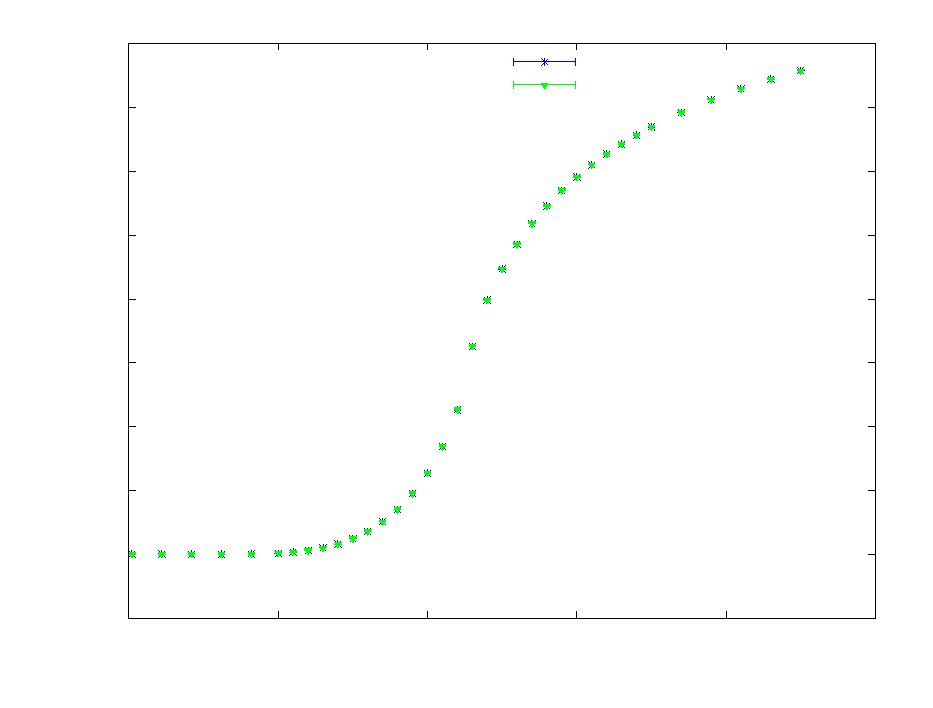
\includegraphics{vergleichham}}%
    \gplfronttext
  \end{picture}%
\endgroup

		\caption[Hamiltonian mit und ohne Parallelisierung]{Hamiltonian mit und ohne Parallelisierung bei verschiedenen Temperaturen gemessen. Die Fehler sind mit Blocklänge 128 bestimmt und so klein, dass sie fast nicht sichtbar sind.}
		\label{fig:vergleichham}
	\end{figure}
	
	Um zu ermitteln, mit wie vielen Cores idealerweise gemessen werden sollte, wurde die Skalierung der sweep-Funktion betrachtet. Hierbei wurde für verschiedene Gitterlängen und Temperaturen die Zeit, die für 1.000 Ausführungen der sweep-Funktion benötigt wurde, gemessen. Von zehn solchen Messungen wurden mittels der Standardschätzer Mittelwert und Varianz gebildet. 
	
	\begin{figure}[htbp]
		\input{Bilder/speeduplaenge}
		\caption[Speedup in Abhängigkeit von der Gitterlänge]{Speedup in Abhängigkeit von der Gitterlänge, Mittelwert über $10 \cdot 1000$ Messungen, gemessen bei $T=\num{0,5}$}
		\label{fig:skalierunglaenge}
	\end{figure}
	
	In Abbildung \ref{fig:skalierunglaenge} ist die Skalierung bei verschiedenen Gitterlängen aufgetragen. Gemessen wurde auf der lcpunode02 des Clusterrechners QBiG. (weitere Werte?).
	
	Bei kleinen Gitterlängen wie $10$ wird die Durchführung durch das Verwenden mehrerer Kerne nicht beschleunigt, der overhead der Parallelisierung verlangsamt die Durchführung sogar noch. Bei etwas größeren Gitterlängen wie z.{}B.{} 40, wird die Funktion mit steigender Anzahl an Kernen erst schneller durchgeführt, ab einer gewissen Zahl an Kernen, hier $6$, überwiegt allerdings der overhead gegenüber der Beschleunigung durch weiteres Parallelisieren und der Speedup wird mit steigender Anzahl der Kerne wieder kleiner. Die Fehler sind hier recht groß, das das Programm nicht lange für die ausführung benötigt, nur ca.{} $\num{0,04}\si{\second}$ bei 5 Kernen, sodass hier die natürlichen Variationen der Kerne aufgrund von Hitze o.{}Ä.{} zu einem großen relativen Fehler führen. Der Maximale Speedup ist $\num{3,4\pm0,6}$ Mit steigender Gitterlänge, hier im Beispiel 70, wird der Overhead im Vergleich zur Rechenzeit geringer, sodass der Speedup mit der Anzahl der Kerne annähernd monoton ansteigt, und bei 12 ein Maximum von $\num{4,76\pm0,94}$.
	Bei größeren Gitterlängen wird der Einfluss der Overheads nochmal geringer, wodurch der Anstieg des Speedups steiler wird und bei Gitterlänge 500 der maximale Speedup, bei $12$ Kernen, $\num{6,32\pm0,15}$ beträgt.
 	
	%Wie man an Bild sieht, ist die Parallelisierung für kleine Gitterlängen sinnlos, es wird nur mehr overhead eingeführt und die benötigte Zeit steigt mit Anzahl der Cores.
	
	%Ab einer gewissen Gitterlänge sinkt die benötigte Rechenzeit mit mehr Cores, sinkt allerdings für mehr Cores, wenn es mehr Overhead gibt. Bei steigender Gitterlänge wird allerdings auch die Laufzeitverbesserung für mehr Cores sichtbar, es bildet sich erst ein Plateau, was für lange Gitterlängen schließlich in eine monoton steigende Funktion übergeht.
	\begin{figure}[htbp]
		\input{Bilder/speeduptemperatur}
		\caption[Speedup in Abhängigkeit von der Temperatur]{Speedup in Abhängigkeit von der Temperatur, Mittelwert über $10 \cdot 1000$ Messungen, gemessen bei Gitterlänge 500}
		\label{fig:skalierungtemp}
	\end{figure}
		
	Wenn man sich die Skalierung bei verschiedenen Temperaturen anguckt, siehe Abb. \ref{fig:skalierungtemp}, gibt es auch hier Unterschiede bei konstanter Gitterlänge: für niedrigere Temperaturen ist die Laufzeit geringer, allerdings der maximale speedup kleiner. Vermutlich kommt dies daher, dass bei niedrigen Temperaturen die Akzeptanzrate geringer ist und somit seltener eine Addition beim Hamiltonian durchgeführt werden muss. Diese Unterschiede entsprechen ungefähr einer Standarabweichung, dies ist allerdings recht gering und selbst beim größten Speedup beträgt der unterschied wischen den Temperaturen nur $\num{0,17}$.
	
	Bei Gitterlängen ab $70$ entspricht das Verhalten des Speedups somit den Erwartungen aus Abschnitt \ref{subsec:openmptheorie}. Da im Folgenden das Verhalten bei großen Gitterlängen betrachtet wird, wird nach Möglichkeit mit der maximalen Anzahl an Kernen gerechnet. Einige Messungen wurden auch auf einem Intel(R) Core(TM) i7-7500U CPU @ 2.70GHz durchgeführt.
	%Insgesamt entspricht somit die Skalierung bei hohen Gitterlängen dem Ahmdahlschen Gesetz.
	%Messungen der Parallelisierung von messen/sweep auf lcpunode02 in QBiG: Bis zu 12 Kerne. Kennwerte von lcpunode02?

	%Parallelisierung Bootstrap?
	
	%Zuerst: Vergleich der verschiedenen sweep-Funktionen: Hamiltonian gleich. Bild.
	
	%Skalierung auf lcpunode2: Vergleich zwei Schleifen/tryflip/Temperaturen?
	%Bild von idealem Code, Skalierung wie erwartet (nach Ahmdahls law?)
	
	In Bild \ref{fig:ergebnisakzeptanzrate} ist die Akzeptanzrate als Funktion von der Temperatur dargestellt. Bei kleinen Temperaturen ist sie null, steigt ab ca. $T=1$ an, hat bei ca. $T=\num{2,2}$ einen Wendepunkt mit Akzeptanzrate ca. $\num{0,2}$ und nähert sich danach asymptotisch dem Wert $1$.
	
	\begin{figure}[htbp]
		% GNUPLOT: LaTeX picture with Postscript
\begingroup
  \makeatletter
  \providecommand\color[2][]{%
    \GenericError{(gnuplot) \space\space\space\@spaces}{%
      Package color not loaded in conjunction with
      terminal option `colourtext'%
    }{See the gnuplot documentation for explanation.%
    }{Either use 'blacktext' in gnuplot or load the package
      color.sty in LaTeX.}%
    \renewcommand\color[2][]{}%
  }%
  \providecommand\includegraphics[2][]{%
    \GenericError{(gnuplot) \space\space\space\@spaces}{%
      Package graphicx or graphics not loaded%
    }{See the gnuplot documentation for explanation.%
    }{The gnuplot epslatex terminal needs graphicx.sty or graphics.sty.}%
    \renewcommand\includegraphics[2][]{}%
  }%
  \providecommand\rotatebox[2]{#2}%
  \@ifundefined{ifGPcolor}{%
    \newif\ifGPcolor
    \GPcolortrue
  }{}%
  \@ifundefined{ifGPblacktext}{%
    \newif\ifGPblacktext
    \GPblacktextfalse
  }{}%
  % define a \g@addto@macro without @ in the name:
  \let\gplgaddtomacro\g@addto@macro
  % define empty templates for all commands taking text:
  \gdef\gplbacktext{}%
  \gdef\gplfronttext{}%
  \makeatother
  \ifGPblacktext
    % no textcolor at all
    \def\colorrgb#1{}%
    \def\colorgray#1{}%
  \else
    % gray or color?
    \ifGPcolor
      \def\colorrgb#1{\color[rgb]{#1}}%
      \def\colorgray#1{\color[gray]{#1}}%
      \expandafter\def\csname LTw\endcsname{\color{white}}%
      \expandafter\def\csname LTb\endcsname{\color{black}}%
      \expandafter\def\csname LTa\endcsname{\color{black}}%
      \expandafter\def\csname LT0\endcsname{\color[rgb]{1,0,0}}%
      \expandafter\def\csname LT1\endcsname{\color[rgb]{0,1,0}}%
      \expandafter\def\csname LT2\endcsname{\color[rgb]{0,0,1}}%
      \expandafter\def\csname LT3\endcsname{\color[rgb]{1,0,1}}%
      \expandafter\def\csname LT4\endcsname{\color[rgb]{0,1,1}}%
      \expandafter\def\csname LT5\endcsname{\color[rgb]{1,1,0}}%
      \expandafter\def\csname LT6\endcsname{\color[rgb]{0,0,0}}%
      \expandafter\def\csname LT7\endcsname{\color[rgb]{1,0.3,0}}%
      \expandafter\def\csname LT8\endcsname{\color[rgb]{0.5,0.5,0.5}}%
    \else
      % gray
      \def\colorrgb#1{\color{black}}%
      \def\colorgray#1{\color[gray]{#1}}%
      \expandafter\def\csname LTw\endcsname{\color{white}}%
      \expandafter\def\csname LTb\endcsname{\color{black}}%
      \expandafter\def\csname LTa\endcsname{\color{black}}%
      \expandafter\def\csname LT0\endcsname{\color{black}}%
      \expandafter\def\csname LT1\endcsname{\color{black}}%
      \expandafter\def\csname LT2\endcsname{\color{black}}%
      \expandafter\def\csname LT3\endcsname{\color{black}}%
      \expandafter\def\csname LT4\endcsname{\color{black}}%
      \expandafter\def\csname LT5\endcsname{\color{black}}%
      \expandafter\def\csname LT6\endcsname{\color{black}}%
      \expandafter\def\csname LT7\endcsname{\color{black}}%
      \expandafter\def\csname LT8\endcsname{\color{black}}%
    \fi
  \fi
    \setlength{\unitlength}{0.0500bp}%
    \ifx\gptboxheight\undefined%
      \newlength{\gptboxheight}%
      \newlength{\gptboxwidth}%
      \newsavebox{\gptboxtext}%
    \fi%
    \setlength{\fboxrule}{0.5pt}%
    \setlength{\fboxsep}{1pt}%
\begin{picture}(8640.00,4320.00)%
    \gplgaddtomacro\gplbacktext{%
      \csname LTb\endcsname%
      \put(1164,737){\makebox(0,0)[r]{\strut{}$0$}}%
      \put(1164,1394){\makebox(0,0)[r]{\strut{}$0.2$}}%
      \put(1164,2051){\makebox(0,0)[r]{\strut{}$0.4$}}%
      \put(1164,2708){\makebox(0,0)[r]{\strut{}$0.6$}}%
      \put(1164,3365){\makebox(0,0)[r]{\strut{}$0.8$}}%
      \put(1164,4022){\makebox(0,0)[r]{\strut{}$1$}}%
      \put(1299,484){\makebox(0,0){\strut{}$0$}}%
      \put(1990,484){\makebox(0,0){\strut{}$2000$}}%
      \put(2680,484){\makebox(0,0){\strut{}$4000$}}%
      \put(3370,484){\makebox(0,0){\strut{}$6000$}}%
      \put(4061,484){\makebox(0,0){\strut{}$8000$}}%
      \put(4751,484){\makebox(0,0){\strut{}$10000$}}%
    }%
    \gplgaddtomacro\gplfronttext{%
      \csname LTb\endcsname%
      \put(526,2379){\rotatebox{-270}{\makebox(0,0){\strut{}Akzeptanzrate}}}%
      \put(3023,154){\makebox(0,0){\strut{}Temperatur}}%
    }%
    \gplgaddtomacro\gplbacktext{%
      \csname LTb\endcsname%
      \put(4620,737){\makebox(0,0)[r]{\strut{}}}%
      \put(4620,1394){\makebox(0,0)[r]{\strut{}}}%
      \put(4620,2051){\makebox(0,0)[r]{\strut{}}}%
      \put(4620,2708){\makebox(0,0)[r]{\strut{}}}%
      \put(4620,3365){\makebox(0,0)[r]{\strut{}}}%
      \put(4620,4022){\makebox(0,0)[r]{\strut{}}}%
      \put(4752,484){\makebox(0,0){\strut{}$0$}}%
      \put(5443,484){\makebox(0,0){\strut{}$1$}}%
      \put(6134,484){\makebox(0,0){\strut{}$2$}}%
      \put(6825,484){\makebox(0,0){\strut{}$3$}}%
      \put(7516,484){\makebox(0,0){\strut{}$4$}}%
      \put(8207,484){\makebox(0,0){\strut{}$5$}}%
    }%
    \gplgaddtomacro\gplfronttext{%
      \csname LTb\endcsname%
      \put(6479,154){\makebox(0,0){\strut{}Temperatur}}%
    }%
    \gplbacktext
    \put(0,0){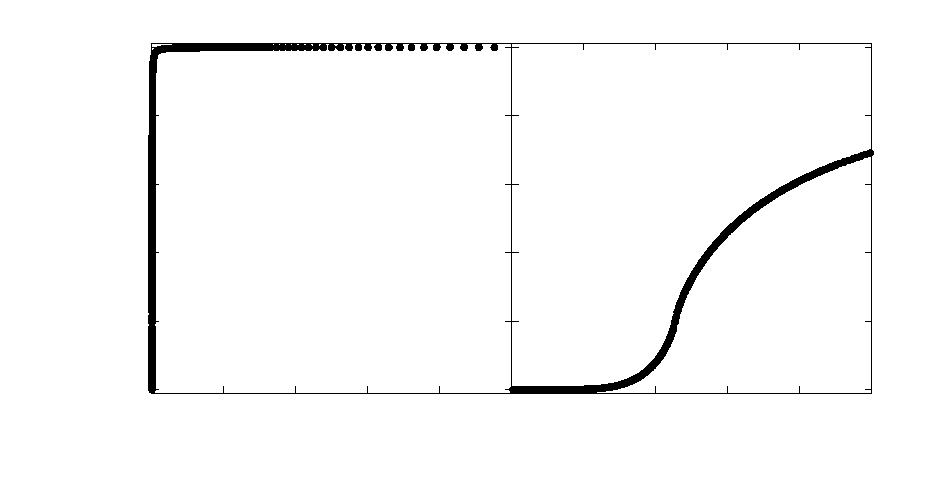
\includegraphics{akzeptanzrate}}%
    \gplfronttext
  \end{picture}%
\endgroup

		\caption[Akzeptanzrate in Abhängigkeit von der Temperatur]{Akzeptanzrate in Abhängigkeit von der Temperatur, gemessen bei Gitterlänge 120, mit Blocklänge 128 zur Fehlerberechnung. Die Fehler sind so klein, dass sie fast nicht sichtbar sind.}
		\label{fig:ergebnisakzeptanzrate}
	\end{figure}
	
	Der Hamiltonian verhält sich qualitativ ähnlich, siehe Bild \ref{fig:ergebnishamiltonian}. Bei geringen Temperaturen hat er den Wert $-2\cdot\text{laenge}^2$, was auf ein vollkommen homogen ausgerichtetes Gitter hinweist. Bei ca T=2,2 beträgt der Hamiltonian ca. $-\num{1,4}\cdot\text{laenge}^2$ und nähert sich dann asymptotisch null.
	
	\begin{figure}[htbp]
		% GNUPLOT: LaTeX picture with Postscript
\begingroup
  \makeatletter
  \providecommand\color[2][]{%
    \GenericError{(gnuplot) \space\space\space\@spaces}{%
      Package color not loaded in conjunction with
      terminal option `colourtext'%
    }{See the gnuplot documentation for explanation.%
    }{Either use 'blacktext' in gnuplot or load the package
      color.sty in LaTeX.}%
    \renewcommand\color[2][]{}%
  }%
  \providecommand\includegraphics[2][]{%
    \GenericError{(gnuplot) \space\space\space\@spaces}{%
      Package graphicx or graphics not loaded%
    }{See the gnuplot documentation for explanation.%
    }{The gnuplot epslatex terminal needs graphicx.sty or graphics.sty.}%
    \renewcommand\includegraphics[2][]{}%
  }%
  \providecommand\rotatebox[2]{#2}%
  \@ifundefined{ifGPcolor}{%
    \newif\ifGPcolor
    \GPcolortrue
  }{}%
  \@ifundefined{ifGPblacktext}{%
    \newif\ifGPblacktext
    \GPblacktextfalse
  }{}%
  % define a \g@addto@macro without @ in the name:
  \let\gplgaddtomacro\g@addto@macro
  % define empty templates for all commands taking text:
  \gdef\gplbacktext{}%
  \gdef\gplfronttext{}%
  \makeatother
  \ifGPblacktext
    % no textcolor at all
    \def\colorrgb#1{}%
    \def\colorgray#1{}%
  \else
    % gray or color?
    \ifGPcolor
      \def\colorrgb#1{\color[rgb]{#1}}%
      \def\colorgray#1{\color[gray]{#1}}%
      \expandafter\def\csname LTw\endcsname{\color{white}}%
      \expandafter\def\csname LTb\endcsname{\color{black}}%
      \expandafter\def\csname LTa\endcsname{\color{black}}%
      \expandafter\def\csname LT0\endcsname{\color[rgb]{1,0,0}}%
      \expandafter\def\csname LT1\endcsname{\color[rgb]{0,1,0}}%
      \expandafter\def\csname LT2\endcsname{\color[rgb]{0,0,1}}%
      \expandafter\def\csname LT3\endcsname{\color[rgb]{1,0,1}}%
      \expandafter\def\csname LT4\endcsname{\color[rgb]{0,1,1}}%
      \expandafter\def\csname LT5\endcsname{\color[rgb]{1,1,0}}%
      \expandafter\def\csname LT6\endcsname{\color[rgb]{0,0,0}}%
      \expandafter\def\csname LT7\endcsname{\color[rgb]{1,0.3,0}}%
      \expandafter\def\csname LT8\endcsname{\color[rgb]{0.5,0.5,0.5}}%
    \else
      % gray
      \def\colorrgb#1{\color{black}}%
      \def\colorgray#1{\color[gray]{#1}}%
      \expandafter\def\csname LTw\endcsname{\color{white}}%
      \expandafter\def\csname LTb\endcsname{\color{black}}%
      \expandafter\def\csname LTa\endcsname{\color{black}}%
      \expandafter\def\csname LT0\endcsname{\color{black}}%
      \expandafter\def\csname LT1\endcsname{\color{black}}%
      \expandafter\def\csname LT2\endcsname{\color{black}}%
      \expandafter\def\csname LT3\endcsname{\color{black}}%
      \expandafter\def\csname LT4\endcsname{\color{black}}%
      \expandafter\def\csname LT5\endcsname{\color{black}}%
      \expandafter\def\csname LT6\endcsname{\color{black}}%
      \expandafter\def\csname LT7\endcsname{\color{black}}%
      \expandafter\def\csname LT8\endcsname{\color{black}}%
    \fi
  \fi
    \setlength{\unitlength}{0.0500bp}%
    \ifx\gptboxheight\undefined%
      \newlength{\gptboxheight}%
      \newlength{\gptboxwidth}%
      \newsavebox{\gptboxtext}%
    \fi%
    \setlength{\fboxrule}{0.5pt}%
    \setlength{\fboxsep}{1pt}%
\begin{picture}(8640.00,4320.00)%
    \gplgaddtomacro\gplbacktext{%
      \csname LTb\endcsname%
      \put(1164,721){\makebox(0,0)[r]{\strut{}$-2$}}%
      \put(1164,1550){\makebox(0,0)[r]{\strut{}$-1.5$}}%
      \put(1164,2380){\makebox(0,0)[r]{\strut{}$-1$}}%
      \put(1164,3209){\makebox(0,0)[r]{\strut{}$-0.5$}}%
      \put(1164,4038){\makebox(0,0)[r]{\strut{}$0$}}%
      \put(1299,484){\makebox(0,0){\strut{}$0$}}%
      \put(1990,484){\makebox(0,0){\strut{}$2000$}}%
      \put(2680,484){\makebox(0,0){\strut{}$4000$}}%
      \put(3370,484){\makebox(0,0){\strut{}$6000$}}%
      \put(4061,484){\makebox(0,0){\strut{}$8000$}}%
      \put(4751,484){\makebox(0,0){\strut{}$10000$}}%
    }%
    \gplgaddtomacro\gplfronttext{%
      \csname LTb\endcsname%
      \put(394,2379){\rotatebox{-270}{\makebox(0,0){\strut{}$H/\text{laenge}^2$}}}%
      \put(3023,154){\makebox(0,0){\strut{}Temperatur}}%
    }%
    \gplgaddtomacro\gplbacktext{%
      \csname LTb\endcsname%
      \put(4620,721){\makebox(0,0)[r]{\strut{}}}%
      \put(4620,1550){\makebox(0,0)[r]{\strut{}}}%
      \put(4620,2380){\makebox(0,0)[r]{\strut{}}}%
      \put(4620,3209){\makebox(0,0)[r]{\strut{}}}%
      \put(4620,4038){\makebox(0,0)[r]{\strut{}}}%
      \put(4752,484){\makebox(0,0){\strut{}$0$}}%
      \put(5443,484){\makebox(0,0){\strut{}$1$}}%
      \put(6134,484){\makebox(0,0){\strut{}$2$}}%
      \put(6825,484){\makebox(0,0){\strut{}$3$}}%
      \put(7516,484){\makebox(0,0){\strut{}$4$}}%
      \put(8207,484){\makebox(0,0){\strut{}$5$}}%
    }%
    \gplgaddtomacro\gplfronttext{%
      \csname LTb\endcsname%
      \put(6479,154){\makebox(0,0){\strut{}Temperatur}}%
    }%
    \gplbacktext
    \put(0,0){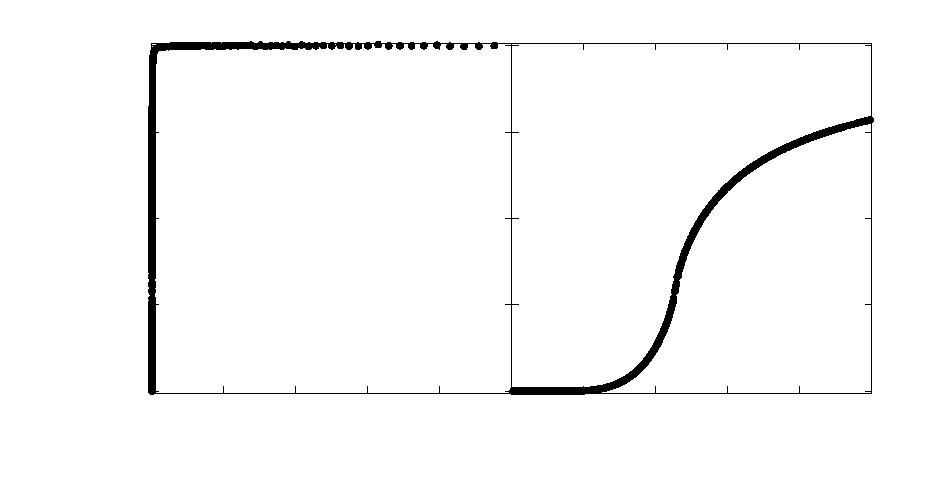
\includegraphics{hamiltonian}}%
    \gplfronttext
  \end{picture}%
\endgroup

		\caption[Hamiltonian in Abhängigkeit von der Temperatur]{Hamiltonian in Abhängigkeit von der Temperatur, gemessen bei Gitterlänge 120, mit Blocklänge 128 zur Fehlerberechnung. Die Fehler sind so klein, dass sie fast nicht sichtbar sind.}
		\label{fig:ergebnishamiltonian}
	\end{figure}
	
%	Dann Akzeptanzrate von wo bis wo, mit gebootstraptem Fehler? Geht auf 1 hoch?
%	\begin{verbatim}
%	test
%	\end{verbatim}

	Die Magnetisierung verhält sich wie nach Gl. \ref{eq:magnetisierungsgleichungliteratur} erwartet: Bei geringen Temperaturen ist sie eins, danach wird sich kleiner. Bei ca. $\num{2,2}$ hat sie einen starken Abfall, und nähert sich danach einem konstanten Wert größer als null an. Nach Gl. \ref{eq:magnetisierungsgleichungliteratur} wäre zu erwarten, dass der Abfall eine scharfe Kante bildet und danach die Magnetisierung null ist, dies ist allerdings aufgrund der endlichen Gittergöße nicht der Fall, wie in~\cite[Abschnitt 2.3.3]{binderheermann} erläutert wird.


	
	\begin{figure}[htbp]
		% GNUPLOT: LaTeX picture with Postscript
\begingroup
  \makeatletter
  \providecommand\color[2][]{%
    \GenericError{(gnuplot) \space\space\space\@spaces}{%
      Package color not loaded in conjunction with
      terminal option `colourtext'%
    }{See the gnuplot documentation for explanation.%
    }{Either use 'blacktext' in gnuplot or load the package
      color.sty in LaTeX.}%
    \renewcommand\color[2][]{}%
  }%
  \providecommand\includegraphics[2][]{%
    \GenericError{(gnuplot) \space\space\space\@spaces}{%
      Package graphicx or graphics not loaded%
    }{See the gnuplot documentation for explanation.%
    }{The gnuplot epslatex terminal needs graphicx.sty or graphics.sty.}%
    \renewcommand\includegraphics[2][]{}%
  }%
  \providecommand\rotatebox[2]{#2}%
  \@ifundefined{ifGPcolor}{%
    \newif\ifGPcolor
    \GPcolortrue
  }{}%
  \@ifundefined{ifGPblacktext}{%
    \newif\ifGPblacktext
    \GPblacktextfalse
  }{}%
  % define a \g@addto@macro without @ in the name:
  \let\gplgaddtomacro\g@addto@macro
  % define empty templates for all commands taking text:
  \gdef\gplbacktext{}%
  \gdef\gplfronttext{}%
  \makeatother
  \ifGPblacktext
    % no textcolor at all
    \def\colorrgb#1{}%
    \def\colorgray#1{}%
  \else
    % gray or color?
    \ifGPcolor
      \def\colorrgb#1{\color[rgb]{#1}}%
      \def\colorgray#1{\color[gray]{#1}}%
      \expandafter\def\csname LTw\endcsname{\color{white}}%
      \expandafter\def\csname LTb\endcsname{\color{black}}%
      \expandafter\def\csname LTa\endcsname{\color{black}}%
      \expandafter\def\csname LT0\endcsname{\color[rgb]{1,0,0}}%
      \expandafter\def\csname LT1\endcsname{\color[rgb]{0,1,0}}%
      \expandafter\def\csname LT2\endcsname{\color[rgb]{0,0,1}}%
      \expandafter\def\csname LT3\endcsname{\color[rgb]{1,0,1}}%
      \expandafter\def\csname LT4\endcsname{\color[rgb]{0,1,1}}%
      \expandafter\def\csname LT5\endcsname{\color[rgb]{1,1,0}}%
      \expandafter\def\csname LT6\endcsname{\color[rgb]{0,0,0}}%
      \expandafter\def\csname LT7\endcsname{\color[rgb]{1,0.3,0}}%
      \expandafter\def\csname LT8\endcsname{\color[rgb]{0.5,0.5,0.5}}%
    \else
      % gray
      \def\colorrgb#1{\color{black}}%
      \def\colorgray#1{\color[gray]{#1}}%
      \expandafter\def\csname LTw\endcsname{\color{white}}%
      \expandafter\def\csname LTb\endcsname{\color{black}}%
      \expandafter\def\csname LTa\endcsname{\color{black}}%
      \expandafter\def\csname LT0\endcsname{\color{black}}%
      \expandafter\def\csname LT1\endcsname{\color{black}}%
      \expandafter\def\csname LT2\endcsname{\color{black}}%
      \expandafter\def\csname LT3\endcsname{\color{black}}%
      \expandafter\def\csname LT4\endcsname{\color{black}}%
      \expandafter\def\csname LT5\endcsname{\color{black}}%
      \expandafter\def\csname LT6\endcsname{\color{black}}%
      \expandafter\def\csname LT7\endcsname{\color{black}}%
      \expandafter\def\csname LT8\endcsname{\color{black}}%
    \fi
  \fi
    \setlength{\unitlength}{0.0500bp}%
    \ifx\gptboxheight\undefined%
      \newlength{\gptboxheight}%
      \newlength{\gptboxwidth}%
      \newsavebox{\gptboxtext}%
    \fi%
    \setlength{\fboxrule}{0.5pt}%
    \setlength{\fboxsep}{1pt}%
\begin{picture}(8640.00,4320.00)%
    \gplgaddtomacro\gplbacktext{%
      \csname LTb\endcsname%
      \put(1164,737){\makebox(0,0)[r]{\strut{}$0$}}%
      \put(1164,1394){\makebox(0,0)[r]{\strut{}$0.2$}}%
      \put(1164,2051){\makebox(0,0)[r]{\strut{}$0.4$}}%
      \put(1164,2708){\makebox(0,0)[r]{\strut{}$0.6$}}%
      \put(1164,3365){\makebox(0,0)[r]{\strut{}$0.8$}}%
      \put(1164,4022){\makebox(0,0)[r]{\strut{}$1$}}%
      \put(1299,484){\makebox(0,0){\strut{}$0$}}%
      \put(1990,484){\makebox(0,0){\strut{}$2000$}}%
      \put(2680,484){\makebox(0,0){\strut{}$4000$}}%
      \put(3370,484){\makebox(0,0){\strut{}$6000$}}%
      \put(4061,484){\makebox(0,0){\strut{}$8000$}}%
      \put(4751,484){\makebox(0,0){\strut{}$10000$}}%
    }%
    \gplgaddtomacro\gplfronttext{%
      \csname LTb\endcsname%
      \put(526,2379){\rotatebox{-270}{\makebox(0,0){\strut{}$M$}}}%
      \put(3023,154){\makebox(0,0){\strut{}Temperatur}}%
    }%
    \gplgaddtomacro\gplbacktext{%
      \csname LTb\endcsname%
      \put(4620,737){\makebox(0,0)[r]{\strut{}}}%
      \put(4620,1394){\makebox(0,0)[r]{\strut{}}}%
      \put(4620,2051){\makebox(0,0)[r]{\strut{}}}%
      \put(4620,2708){\makebox(0,0)[r]{\strut{}}}%
      \put(4620,3365){\makebox(0,0)[r]{\strut{}}}%
      \put(4620,4022){\makebox(0,0)[r]{\strut{}}}%
      \put(4752,484){\makebox(0,0){\strut{}$0$}}%
      \put(5443,484){\makebox(0,0){\strut{}$1$}}%
      \put(6134,484){\makebox(0,0){\strut{}$2$}}%
      \put(6825,484){\makebox(0,0){\strut{}$3$}}%
      \put(7516,484){\makebox(0,0){\strut{}$4$}}%
      \put(8207,484){\makebox(0,0){\strut{}$5$}}%
    }%
    \gplgaddtomacro\gplfronttext{%
      \csname LTb\endcsname%
      \put(6479,154){\makebox(0,0){\strut{}Temperatur}}%
    }%
    \gplbacktext
    \put(0,0){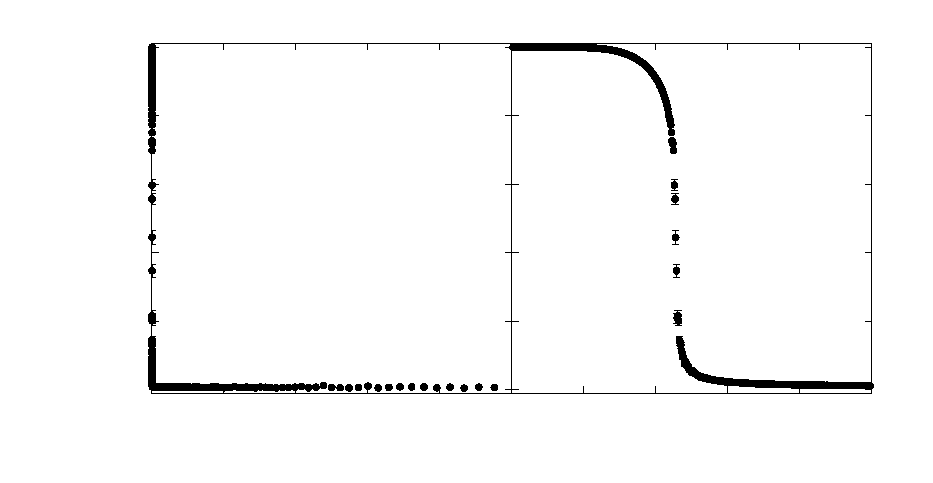
\includegraphics{magnetisierung}}%
    \gplfronttext
  \end{picture}%
\endgroup

		\caption[Magnetisierung in Abhängigkeit von der Temperatur]{Magnetisierung in Abhängigkeit von der Temperatur, gemessen bei Gitterlänge 120, mit Blocklänge 128 zur Fehlerberechnung. Die Fehler sind teilweise so klein, dass sie fast nicht sichtbar sind.}
		\label{fig:ergebnismagnetisierung}
	\end{figure}	
	
	%Dann Magnetisierung: Vergleich zweier Längen, Erklärung finite size Effekts wie in Binder-Heermann erwähnt.

	In Bild \ref{fig:ergebnismagnetisierung} ist dieses Verhalten zu sehen. In Bild \ref{fig:maglaenge} ist dies noch deutlicher zu sehen, dort wird die Magnetisierung bei zwei verschiedenen Längen miteinander verglichen. Es fällt auf, dass bei kleineren Längen der Abfall der Magnetisierung weniger steil ist, sowie die Magnetisierung oberhalb des kritischen Punktes einen größeren Wert hat. Auch dies deckt sich mit den Erwartungen aus~\cite[Abschnitt 2.3.3]{binderheermann}.%, ebenso wie der Vergleich zweier Längen: bei kleineren Gitterlängen ist der Abfall weniger steil und der Wert der Magnetisierung bei hohen Temperaturen größer.

	
	
	\begin{figure}[htbp]
		% GNUPLOT: LaTeX picture with Postscript
\begingroup
  \makeatletter
  \providecommand\color[2][]{%
    \GenericError{(gnuplot) \space\space\space\@spaces}{%
      Package color not loaded in conjunction with
      terminal option `colourtext'%
    }{See the gnuplot documentation for explanation.%
    }{Either use 'blacktext' in gnuplot or load the package
      color.sty in LaTeX.}%
    \renewcommand\color[2][]{}%
  }%
  \providecommand\includegraphics[2][]{%
    \GenericError{(gnuplot) \space\space\space\@spaces}{%
      Package graphicx or graphics not loaded%
    }{See the gnuplot documentation for explanation.%
    }{The gnuplot epslatex terminal needs graphicx.sty or graphics.sty.}%
    \renewcommand\includegraphics[2][]{}%
  }%
  \providecommand\rotatebox[2]{#2}%
  \@ifundefined{ifGPcolor}{%
    \newif\ifGPcolor
    \GPcolortrue
  }{}%
  \@ifundefined{ifGPblacktext}{%
    \newif\ifGPblacktext
    \GPblacktextfalse
  }{}%
  % define a \g@addto@macro without @ in the name:
  \let\gplgaddtomacro\g@addto@macro
  % define empty templates for all commands taking text:
  \gdef\gplbacktext{}%
  \gdef\gplfronttext{}%
  \makeatother
  \ifGPblacktext
    % no textcolor at all
    \def\colorrgb#1{}%
    \def\colorgray#1{}%
  \else
    % gray or color?
    \ifGPcolor
      \def\colorrgb#1{\color[rgb]{#1}}%
      \def\colorgray#1{\color[gray]{#1}}%
      \expandafter\def\csname LTw\endcsname{\color{white}}%
      \expandafter\def\csname LTb\endcsname{\color{black}}%
      \expandafter\def\csname LTa\endcsname{\color{black}}%
      \expandafter\def\csname LT0\endcsname{\color[rgb]{1,0,0}}%
      \expandafter\def\csname LT1\endcsname{\color[rgb]{0,1,0}}%
      \expandafter\def\csname LT2\endcsname{\color[rgb]{0,0,1}}%
      \expandafter\def\csname LT3\endcsname{\color[rgb]{1,0,1}}%
      \expandafter\def\csname LT4\endcsname{\color[rgb]{0,1,1}}%
      \expandafter\def\csname LT5\endcsname{\color[rgb]{1,1,0}}%
      \expandafter\def\csname LT6\endcsname{\color[rgb]{0,0,0}}%
      \expandafter\def\csname LT7\endcsname{\color[rgb]{1,0.3,0}}%
      \expandafter\def\csname LT8\endcsname{\color[rgb]{0.5,0.5,0.5}}%
    \else
      % gray
      \def\colorrgb#1{\color{black}}%
      \def\colorgray#1{\color[gray]{#1}}%
      \expandafter\def\csname LTw\endcsname{\color{white}}%
      \expandafter\def\csname LTb\endcsname{\color{black}}%
      \expandafter\def\csname LTa\endcsname{\color{black}}%
      \expandafter\def\csname LT0\endcsname{\color{black}}%
      \expandafter\def\csname LT1\endcsname{\color{black}}%
      \expandafter\def\csname LT2\endcsname{\color{black}}%
      \expandafter\def\csname LT3\endcsname{\color{black}}%
      \expandafter\def\csname LT4\endcsname{\color{black}}%
      \expandafter\def\csname LT5\endcsname{\color{black}}%
      \expandafter\def\csname LT6\endcsname{\color{black}}%
      \expandafter\def\csname LT7\endcsname{\color{black}}%
      \expandafter\def\csname LT8\endcsname{\color{black}}%
    \fi
  \fi
    \setlength{\unitlength}{0.0500bp}%
    \ifx\gptboxheight\undefined%
      \newlength{\gptboxheight}%
      \newlength{\gptboxwidth}%
      \newsavebox{\gptboxtext}%
    \fi%
    \setlength{\fboxrule}{0.5pt}%
    \setlength{\fboxsep}{1pt}%
\begin{picture}(8640.00,6480.00)%
    \gplgaddtomacro\gplbacktext{%
      \csname LTb\endcsname%
      \put(1164,1296){\makebox(0,0)[r]{\strut{}$0$}}%
      \put(1164,2268){\makebox(0,0)[r]{\strut{}$0.2$}}%
      \put(1164,3240){\makebox(0,0)[r]{\strut{}$0.4$}}%
      \put(1164,4211){\makebox(0,0)[r]{\strut{}$0.6$}}%
      \put(1164,5183){\makebox(0,0)[r]{\strut{}$0.8$}}%
      \put(1164,6155){\makebox(0,0)[r]{\strut{}$1$}}%
      \put(1296,1076){\makebox(0,0){\strut{}$1$}}%
      \put(2448,1076){\makebox(0,0){\strut{}$1.5$}}%
      \put(3600,1076){\makebox(0,0){\strut{}$2$}}%
      \put(4752,1076){\makebox(0,0){\strut{}$2.5$}}%
      \put(5903,1076){\makebox(0,0){\strut{}$3$}}%
      \put(7055,1076){\makebox(0,0){\strut{}$3.5$}}%
      \put(8207,1076){\makebox(0,0){\strut{}$4$}}%
    }%
    \gplgaddtomacro\gplfronttext{%
      \csname LTb\endcsname%
      \put(526,3725){\rotatebox{-270}{\makebox(0,0){\strut{}$M$}}}%
      \put(4751,746){\makebox(0,0){\strut{}Temperatur}}%
      \csname LTb\endcsname%
      \put(7220,5982){\makebox(0,0)[r]{\strut{}$\text{laenge}=120$}}%
      \csname LTb\endcsname%
      \put(7220,5762){\makebox(0,0)[r]{\strut{}$\text{laenge}=36$}}%
      \csname LTb\endcsname%
      \put(7220,5542){\makebox(0,0)[r]{\strut{}Theorie}}%
    }%
    \gplbacktext
    \put(0,0){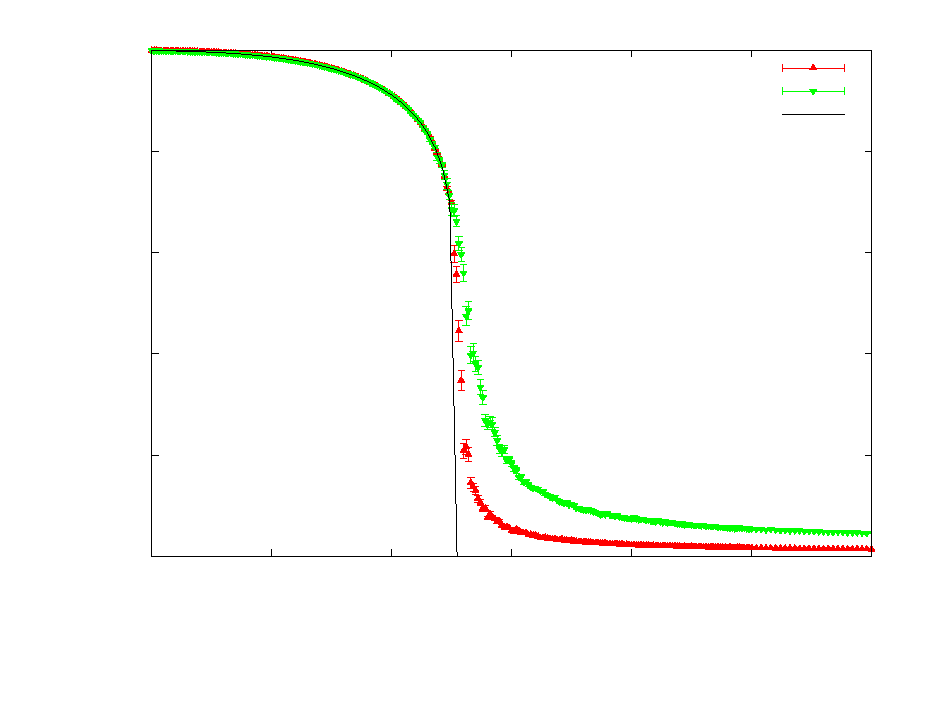
\includegraphics{magnetisierunglaenge}}%
    \gplfronttext
  \end{picture}%
\endgroup

		\caption[Magnetisierung bei verschiedenen Längen]{Magnetisierung bei verschiedenen Längen, Fehler gemessen mit Blocklänge 128}
		\label{fig:maglaenge}
	\end{figure}

	\begin{figure}[htbp]
		% GNUPLOT: LaTeX picture with Postscript
\begingroup
  \makeatletter
  \providecommand\color[2][]{%
    \GenericError{(gnuplot) \space\space\space\@spaces}{%
      Package color not loaded in conjunction with
      terminal option `colourtext'%
    }{See the gnuplot documentation for explanation.%
    }{Either use 'blacktext' in gnuplot or load the package
      color.sty in LaTeX.}%
    \renewcommand\color[2][]{}%
  }%
  \providecommand\includegraphics[2][]{%
    \GenericError{(gnuplot) \space\space\space\@spaces}{%
      Package graphicx or graphics not loaded%
    }{See the gnuplot documentation for explanation.%
    }{The gnuplot epslatex terminal needs graphicx.sty or graphics.sty.}%
    \renewcommand\includegraphics[2][]{}%
  }%
  \providecommand\rotatebox[2]{#2}%
  \@ifundefined{ifGPcolor}{%
    \newif\ifGPcolor
    \GPcolortrue
  }{}%
  \@ifundefined{ifGPblacktext}{%
    \newif\ifGPblacktext
    \GPblacktextfalse
  }{}%
  % define a \g@addto@macro without @ in the name:
  \let\gplgaddtomacro\g@addto@macro
  % define empty templates for all commands taking text:
  \gdef\gplbacktext{}%
  \gdef\gplfronttext{}%
  \makeatother
  \ifGPblacktext
    % no textcolor at all
    \def\colorrgb#1{}%
    \def\colorgray#1{}%
  \else
    % gray or color?
    \ifGPcolor
      \def\colorrgb#1{\color[rgb]{#1}}%
      \def\colorgray#1{\color[gray]{#1}}%
      \expandafter\def\csname LTw\endcsname{\color{white}}%
      \expandafter\def\csname LTb\endcsname{\color{black}}%
      \expandafter\def\csname LTa\endcsname{\color{black}}%
      \expandafter\def\csname LT0\endcsname{\color[rgb]{1,0,0}}%
      \expandafter\def\csname LT1\endcsname{\color[rgb]{0,1,0}}%
      \expandafter\def\csname LT2\endcsname{\color[rgb]{0,0,1}}%
      \expandafter\def\csname LT3\endcsname{\color[rgb]{1,0,1}}%
      \expandafter\def\csname LT4\endcsname{\color[rgb]{0,1,1}}%
      \expandafter\def\csname LT5\endcsname{\color[rgb]{1,1,0}}%
      \expandafter\def\csname LT6\endcsname{\color[rgb]{0,0,0}}%
      \expandafter\def\csname LT7\endcsname{\color[rgb]{1,0.3,0}}%
      \expandafter\def\csname LT8\endcsname{\color[rgb]{0.5,0.5,0.5}}%
    \else
      % gray
      \def\colorrgb#1{\color{black}}%
      \def\colorgray#1{\color[gray]{#1}}%
      \expandafter\def\csname LTw\endcsname{\color{white}}%
      \expandafter\def\csname LTb\endcsname{\color{black}}%
      \expandafter\def\csname LTa\endcsname{\color{black}}%
      \expandafter\def\csname LT0\endcsname{\color{black}}%
      \expandafter\def\csname LT1\endcsname{\color{black}}%
      \expandafter\def\csname LT2\endcsname{\color{black}}%
      \expandafter\def\csname LT3\endcsname{\color{black}}%
      \expandafter\def\csname LT4\endcsname{\color{black}}%
      \expandafter\def\csname LT5\endcsname{\color{black}}%
      \expandafter\def\csname LT6\endcsname{\color{black}}%
      \expandafter\def\csname LT7\endcsname{\color{black}}%
      \expandafter\def\csname LT8\endcsname{\color{black}}%
    \fi
  \fi
    \setlength{\unitlength}{0.0500bp}%
    \ifx\gptboxheight\undefined%
      \newlength{\gptboxheight}%
      \newlength{\gptboxwidth}%
      \newsavebox{\gptboxtext}%
    \fi%
    \setlength{\fboxrule}{0.5pt}%
    \setlength{\fboxsep}{1pt}%
\begin{picture}(8640.00,6480.00)%
    \gplgaddtomacro\gplbacktext{%
      \csname LTb\endcsname%
      \put(1164,1296){\makebox(0,0)[r]{\strut{}$-18$}}%
      \put(1164,1738){\makebox(0,0)[r]{\strut{}$-16$}}%
      \put(1164,2179){\makebox(0,0)[r]{\strut{}$-14$}}%
      \put(1164,2621){\makebox(0,0)[r]{\strut{}$-12$}}%
      \put(1164,3063){\makebox(0,0)[r]{\strut{}$-10$}}%
      \put(1164,3505){\makebox(0,0)[r]{\strut{}$-8$}}%
      \put(1164,3946){\makebox(0,0)[r]{\strut{}$-6$}}%
      \put(1164,4388){\makebox(0,0)[r]{\strut{}$-4$}}%
      \put(1164,4830){\makebox(0,0)[r]{\strut{}$-2$}}%
      \put(1164,5272){\makebox(0,0)[r]{\strut{}$0$}}%
      \put(1164,5713){\makebox(0,0)[r]{\strut{}$2$}}%
      \put(1164,6155){\makebox(0,0)[r]{\strut{}$4$}}%
      \put(1296,1076){\makebox(0,0){\strut{}$1$}}%
      \put(2448,1076){\makebox(0,0){\strut{}$1.5$}}%
      \put(3600,1076){\makebox(0,0){\strut{}$2$}}%
      \put(4752,1076){\makebox(0,0){\strut{}$2.5$}}%
      \put(5903,1076){\makebox(0,0){\strut{}$3$}}%
      \put(7055,1076){\makebox(0,0){\strut{}$3.5$}}%
      \put(8207,1076){\makebox(0,0){\strut{}$4$}}%
    }%
    \gplgaddtomacro\gplfronttext{%
      \csname LTb\endcsname%
      \put(526,3725){\rotatebox{-270}{\makebox(0,0){\strut{}$\dpd{M}{T}$}}}%
      \put(4751,746){\makebox(0,0){\strut{}Temperatur}}%
    }%
    \gplbacktext
    \put(0,0){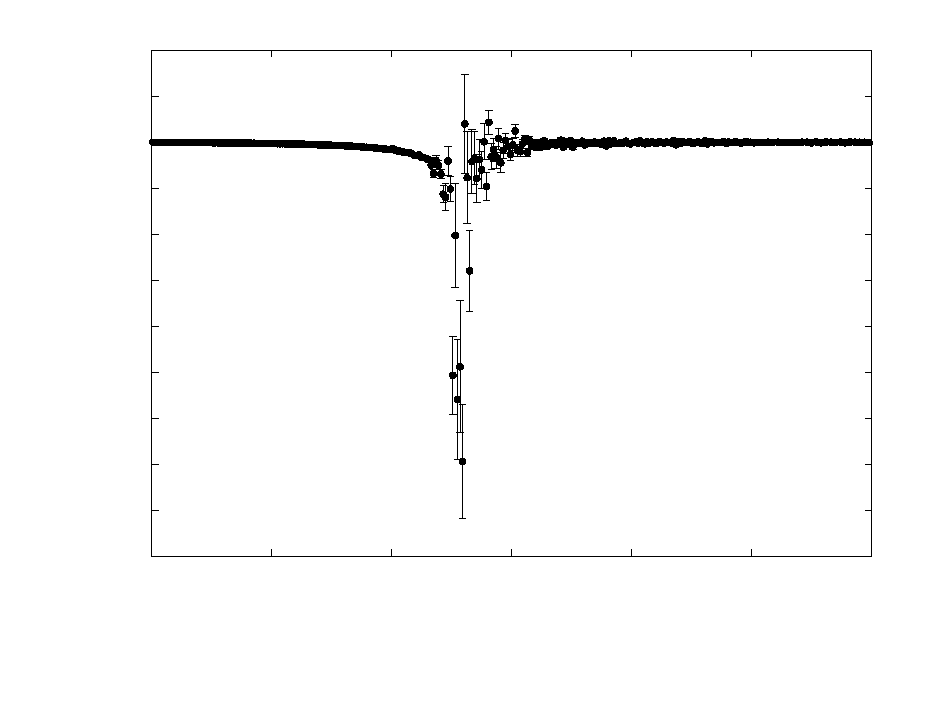
\includegraphics{ableitung120128}}%
    \gplfronttext
  \end{picture}%
\endgroup

		\caption[Ableitung der Magnetisierung]{Ableitung der Magnetisierung, berechnet mit Zwei-Punkt-Formel. Fehler mit Gaußscher Fehlerfortpflanzung aus den Fehlern bei Blocklänge 128 bestimmt}
		\label{fig:ableitung120128}
	\end{figure}
	
	In Bild \ref{fig:maglaenge} ist zusätzlich die nach Gl. \ref{eq:magnetisierungsgleichungliteratur} erwartete Magnetisierung eingezeichnet. Bis zum theoretischen kritischen Punkt, nach Gl. \ref{eq:kritischetemperatur} bei $T=\num{2,269}$, liegen alle Messdaten in ihren Fehlergrenzen auf der erwarteten Kurve, erst danach kommt es aufgrund des weniger starken Abfalls zu Abweichungen.
	
	Um den kritischen Punkt genauer zu bestimmen, wird zusätzlich mit der Zei-Punkt-Formel die Ableitung der gemessenen Magnetisierung bestimmt, siehe Bild \ref{fig:ableitung120128}. Dort wird sichtbar, dass die Änderungsrate der Magnetisierung meist sehr klein ist, nur um den kritischenb Punkt herum ist sie groß.% Die größte Änderung fand im Intervall $2,285\pm0,1$ statt, dies ist minimal größer als der theoretisch erwartete kritische Punkt, die Abweichung beträgt $1,5 \sigma$. 
%	Vergleich gemessene/theoretische Magnetisierung: Nur graphisch oder auch Rechnerisch: Anpassung an Bereich mit Fehlern != 0?
	%Größte Ableitung bei 2,285 pm 0,1 bei Länge 120.
	
	%Bestimmung kritischer Punkt? Über ableitung? Oder Kumulante wie in Binder/Herrmann?
	%Theoretischer Kritischer Punkt: J*2,269
%	Messungen mit QBiG, bei denen nur die Zeit zum Durchführen von 1000 Messungen bei verschiedenen Längen und mit verschieden vielen benutzten Kernen gemessen wurde, zeigen, dass bei kleinen Längen wie 10 die benötigte Zeit mit Anzahl der Kerne sogar zunimmt. Dies ist auf den Overhead zurückzuführen.
%		
%	
%	Messungen auf Intel(R) Core(TM) i7-7500U CPU @ 2.70GHz, lcpunode01 und lcpunode02 auf QBiG.
% Uncomment the following command to get references per chapter.
% Put it inside the file or change \include to \input if you do not want the references
% on a separate page
% \printbibliography[heading=subbibliography]

%------------------------------------------------------------------------------
% Use biblatex for the bibliography
% Add bibliography to Table of Contents
% Comment out this command if your references are printed for each chapter.
\printbibliography[heading=bibintoc]

%------------------------------------------------------------------------------
% Include the following lines and comment out \printbibliography if
% you use BiBTeX for the bibliography.
% If you use biblatex package the files should be specified in the preamble.
% \KOMAoptions{toc=bibliography}
% {\raggedright
%   \bibliographystyle{../refs/atlasBibStyleWithTitle.bst}
%   % \bibliographystyle{unsrt}
%   \bibliography{./thesis_refs,../refs/standard_refs-bibtex}
% }

%------------------------------------------------------------------------------
\appendix
% \part*{Appendix}
% Add your appendices here - don't forget to also add them to \includeonly above
%%------------------------------------------------------------------------------
\chapter{Useful information}
\label{sec:app}
%------------------------------------------------------------------------------

In the appendix you usually include extra information that should be
documented in your thesis, but not interrupt the flow.

%%% Local Variables: 
%%% mode: latex
%%% TeX-master: "../mythesis"
%%% End: 

% \printbibliography[heading=subbibliography]

%------------------------------------------------------------------------------
% Declare lists of figures and tables and acknowledgements as backmatter
% Chapter/section numbers are turned off
\backmatter

\listoffigures
\listoftables

%------------------------------------------------------------------------------
% Print the glossary and list of acronyms
% \printglossaries

%------------------------------------------------------------------------------
% You could instead add your acknowledgements here - don't forget to
% also add them to \includeonly above
% %------------------------------------------------------------------------------
\chapter*{Acknowledgements}
\label{sec:ack}
%------------------------------------------------------------------------------

I would like to thank ...

You should probably use \texttt{\textbackslash chapter*} for
acknowledgements at the beginning of a thesis and
\texttt{\textbackslash chapter} for the end.

%%% Local Variables: 
%%% mode: latex
%%% TeX-master: "../mythesis"
%%% End: 


%------------------------------------------------------------------------------
% CV needed when you submit your PhD thesis
% \input{thesis_cv}

\end{document}

%%% Local Variables:
%%% mode: latex
%%% TeX-master: t
%%% End:
